\documentclass[12pt]{article}
\usepackage[letterpaper,top=2cm,bottom=2cm,left=1.8cm,right=1.8cm,marginparwidth=1.75cm]{geometry}
\usepackage{graphicx} % Required for inserting images
\usepackage[english]{babel}
\usepackage[T1]{fontenc}
\usepackage{listings}
\usepackage{float}
%\%\%usepackage[nomarkers]{endfloat}
\usepackage{color}
\usepackage{xcolor}
\usepackage{tikzducks}
\usepackage{lipsum}
\usepackage{amsmath,amsthm}
\usepackage{amssymb}
\usepackage{isomath}
\usepackage{changepage}
\usepackage{algorithm}
\usepackage{algpseudocode}
\usepackage{colortbl}
\usepackage{caption} 
\usepackage{array}
\usepackage{multicol} % Pour les colonnes
\usepackage[hidelinks]{hyperref}
\usepackage{csquotes}
\usepackage{tikz}
\usepackage[
backend=biber,
style=numeric
]{biblatex}
\addbibresource{biblio.bib}


\newcommand{\K}{\mathbb{K}}
\newcommand{\N}{\mathbb{N}}
\newcommand{\C}{\mathbb{C}}
\newcommand{\R}{\mathbb{R}}
\newcommand{\Rd}{\mathbb{R}^d}
\newcommand{\I}{\mathbf{I}}
\newcommand{\dcrochetg}{[\![}
\newcommand{\dcrochetd}{]\!]}
\newcommand\independent{\protect\mathpalette{\protect\independenT}{\perp}}
\def\independenT#1#2{\mathrel{\rlap{$#1#2$}\mkern2mu{#1#2}}}

%Gary's stuff 
\newtheorem{thm1}{Théorème}[section]
\newtheorem{lemme1}[thm1]{Lemme}
\newtheorem{prop1}[thm1]{Proposition}
\newtheorem*{rmq1}{Remarque}
\newtheorem*{exemple1}{Exemple}
\newtheorem*{defin1}{Définition}
%End of Gary's stuff


\begin{document}
\title{How to classify responses to adversity: resilience and vulnerability as deviations from the average}
\author{Garance Malnoë under the supervision of Jan Höltge}
\date{May - July 2025}

\pagenumbering{gobble}
\maketitle
\tableofcontents
\clearpage
\pagenumbering{arabic}
\section{Introduction / Main Contribution}

The main contribution of this work is the introduction of new classification methods to analyse individual responses to adversity in the context of resilience research. These methods offer a shift in perspective by conceptualising resilience and vulnerability as deviations from the norm. We propose to identify resilient and vulnerable individuals as those whose outcomes are notably better or worse, respectively, than the typical response to a given level of adversity.\\
\\
With this framework, we provide tools to classify individuals into three groups based on the residuals of a regression between an adversity and an outcome: an average or normative group, consisting of individuals whose response is close to the expected or mean response for their level of adversity, a resilient group, whose outcomes are better than expected, and a vulnerable group, whose outcomes are worse.\\
\\
Our approach is designed to be flexible and generalizable: all methods can be implemented using open-source standard statistical tools in R, and they are applicable across a wide range of settings and resilience constructs.\\
\\
In the context of cross-sectional data, we present different approaches to define thresholds of deviation, including approaches based on quantiles, confidence intervals, prediction intervals, credibility intervals, standard deviation, and the k-means algorithm.\\
\\
We extend this framework to longitudinal data using a Bayesian mixed-effects model with spike-and-slab priors for random effect selection. This allows us to identify individuals whose response systematically deviates from the average pattern, again classifying them as resilient, vulnerable, or average depending on the direction and significance of the deviation.\\
\\
This document will be separated into two parts. First, we introduce multiple cross-sectional classification methods based on the residuals of a linear regression between an adversity variable and an outcome variable, where, to ensure robustness, we systematically identify and exclude from the fitting overly influential individuals using standard influence diagnostics. We then present the results of these classification methods on a real-world dataset and assess the relevance of each method by evaluating how well the resulting classification supports predictive modelling. Second, we extend the framework to longitudinal data by modelling the residuals of multiple regressions over time with a mixed-effects approach and present the spike-and-slab methodology to detect persistent deviations from the normative response. Then, we illustrate this method on the same real-world dataset. Both illustrations are fully implemented with open-source tools in R.

\section{Cross-sectional Analysis}
\subsection{Methods}
\subsubsection{Overview}
In the cross-sectional setting, our objective is to identify individuals whose outcomes deviate from the average response to adversity evaluated at a single point in time.\\
\\
To do so, we begin by fitting a linear regression model in which an outcome variable (e.g., a psychological functioning score) is regressed on an adversity variable (e.g., a cumulative adversity index). The residuals from this model capture individual deviations from the expected response, given the observed level of adversity.\\
\\
To ensure that the fitted model is not unduly influenced by some individuals, we use influence diagnostics, specifically Cook's distance, to identify overly influential individuals. These individuals are excluded from the model fitting, but we still compute their residuals from the fitted model for completeness.\\
\\
Finally, individuals are classified into three groups (resilient, average, vulnerable) based on the distribution of residuals, using one of several methods introduced in the classification methods definition section.

\subsubsection{Residualisation}
The first step of the method consists in a residualization, a commonly used method, where where an outcome variable is linearly regressed on an adversity variable. Formally, the model is written as:
\[
\vectorsym{y} = \matrixsym{X}\vectorsym{\hat\beta} + \vectorsym{\epsilon}\\
\]
Where \( \vectorsym{y} \in \mathbb{R}^n \) is the vector of outcomes, \( \matrixsym{X} \in \mathcal{M}_{n,2}(\R) \) is the design matrix with a column of ones and a column containing the adversity scores, \( \vectorsym{\hat\beta} \in \mathbb{R}^2 \) is the vector containing the intercept and slope coefficients, and \( \vectorsym{\epsilon} \in \mathbb{R}^n \) is the vector containing the residuals. The residual for each individual corresponds to the difference between their observed outcome and the predicted outcome given their level of adversity.\\
\\
It's worth noting that the direction of the association between adversity and outcome varies depending on the choice of variables. Thus, the sign of the residuals must be interpreted in context: when a higher outcome score means better functioning, a positive residual reflects a better outcome whereas when a higher outcome means worse functining, a positive residual reflects a worse outcome, as you can see in Figure \ref{fig:interpretation_sign_residuals}.
\begin{figure}[H]
    \centering
    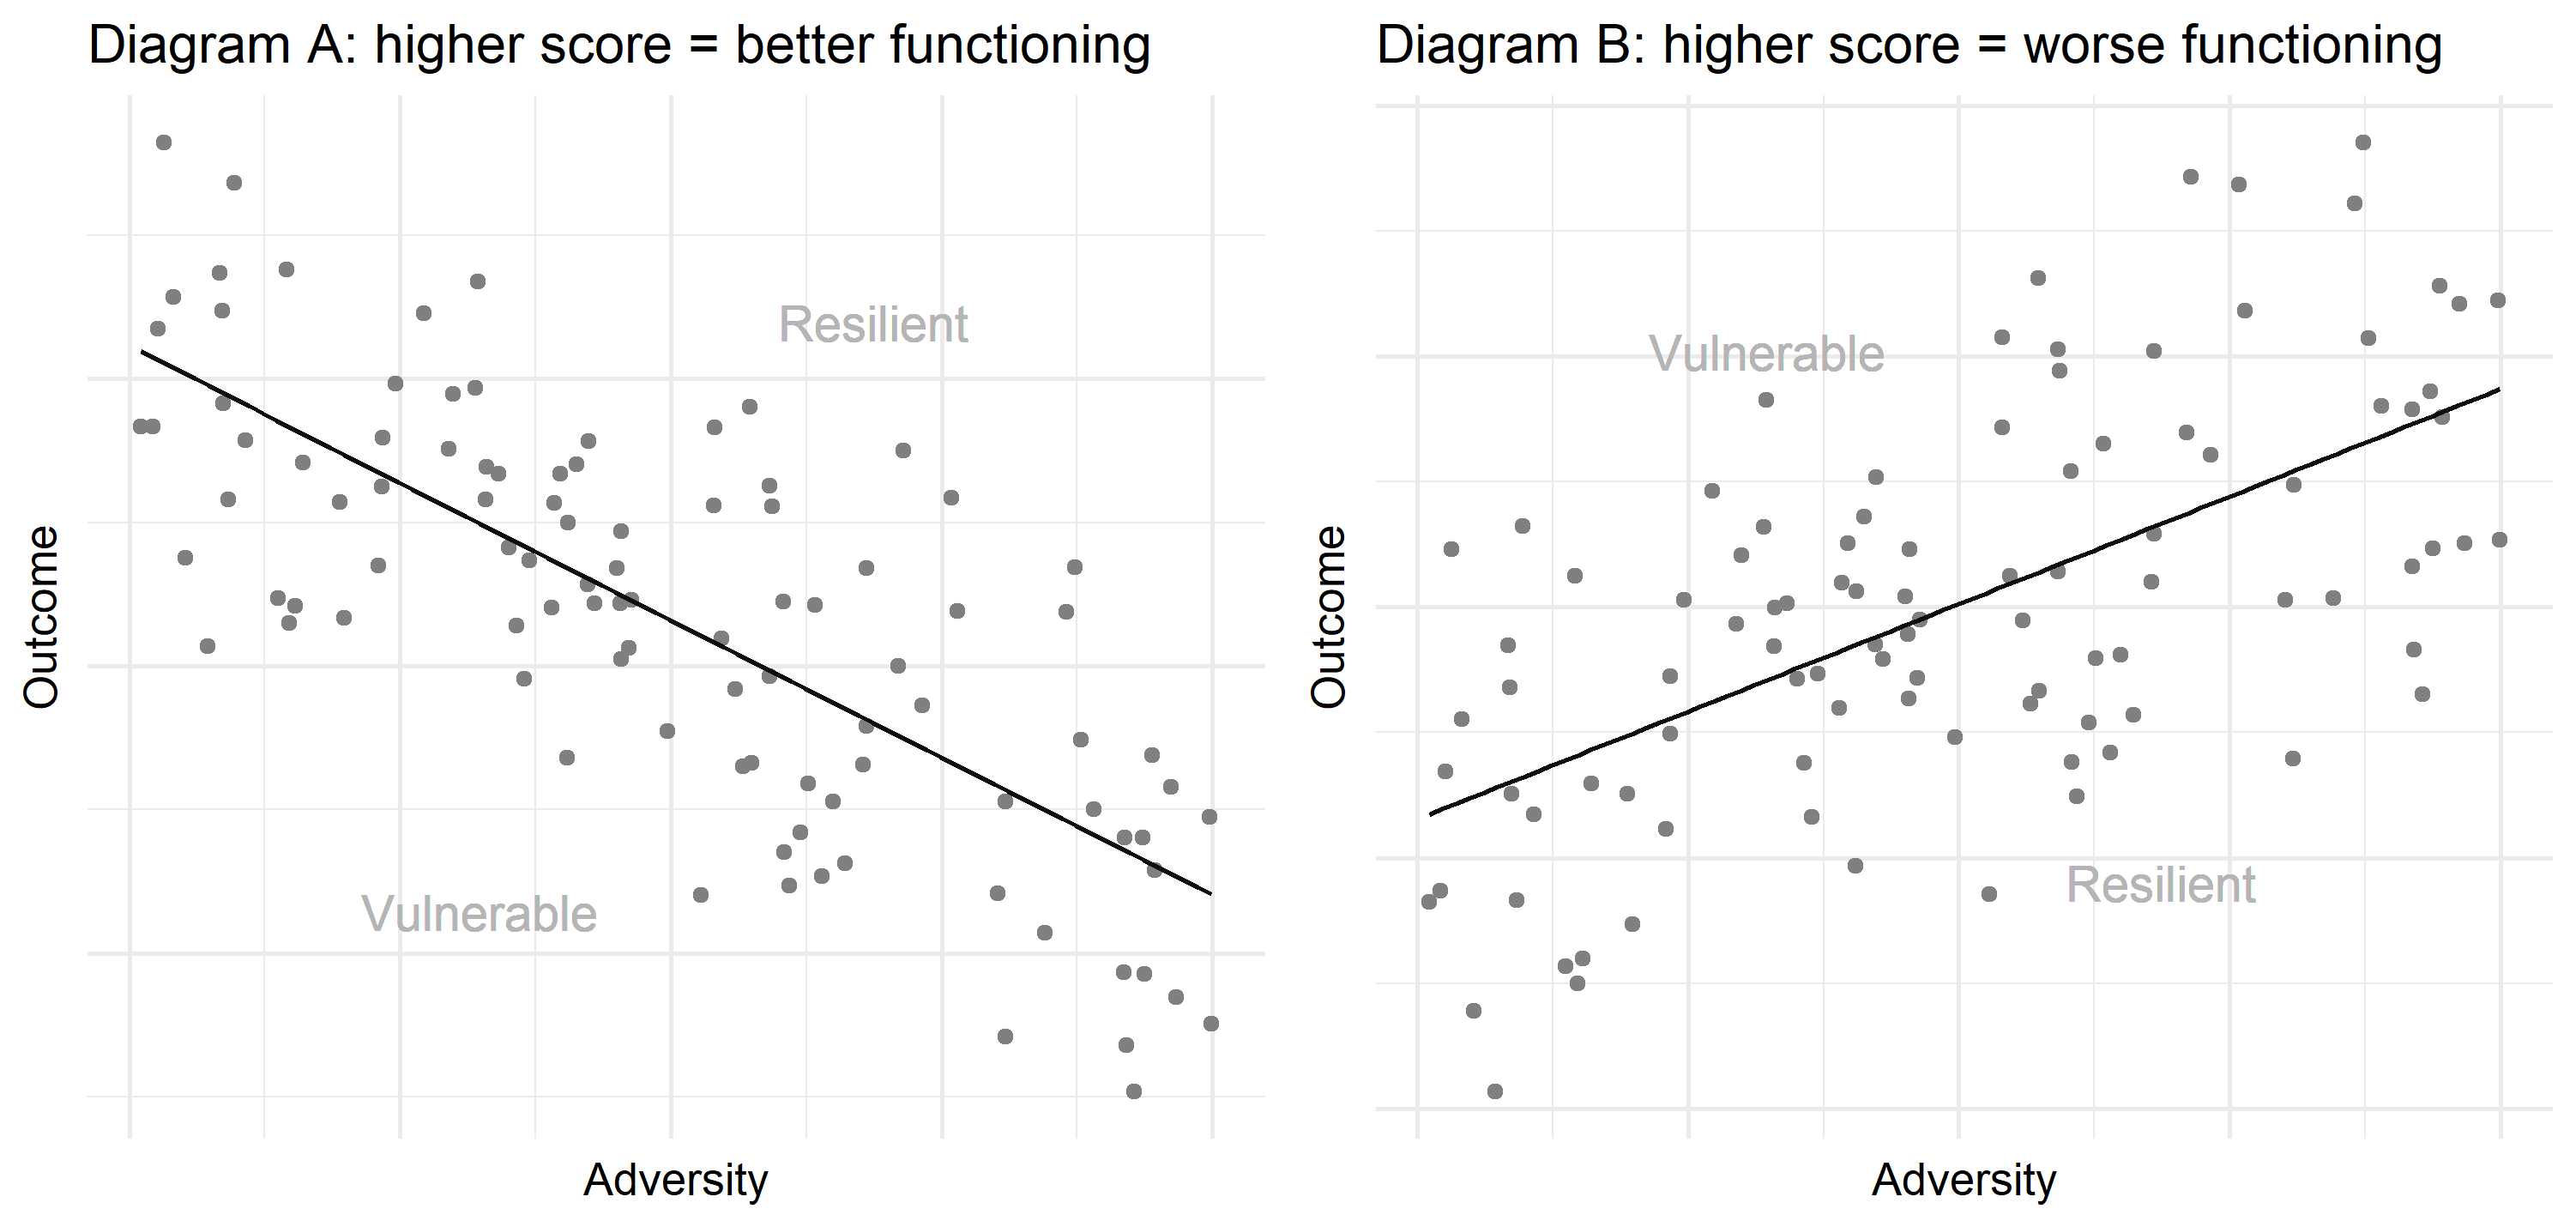
\includegraphics[width=18cm]{Pictures/Diagram_placement_vulnerable_resilient.png}
    \caption{Diagrams explaining the meaning of a residual depending on its sign and the direction of the regression}
    \label{fig:interpretation_sign_residuals}
\end{figure}
\subsubsection{Influence statistics}
To ensure robustness in the estimation of the regression model, we apply influence diagnostics to identify and exclude overly influential individuals. Following the recommendations of \cite{influencial_stat_residuals}, we inspect each individual's Cook's distance, which quantifies the impact of removing that individual on the estimated regression coefficients. Cook's distance is defined as:
\[
D_j = \frac{(\boldsymbol{\hat\beta} - \boldsymbol{\hat\beta}_{(j)})^\top \mathbf{X}^\top \mathbf{X} (\boldsymbol{\hat\beta} - \boldsymbol{\hat\beta}_{(j)})}{p s^2}\\
\]
where \( \boldsymbol{\hat\beta} \) is the vector of estimated coefficients using the full dataset, \( \boldsymbol{\hat\beta}_{(j)} \) is the coefficient vector estimated without the $j^{th}$ individual, \( \mathbf{X} \) is the design matrix, \( p \) is the number of parameters in the model (i.e., the rank of \( \mathbf{X} \)), and \( s^2 \) is the mean squared error of the full model.\\
\\
Individuals with a Cook’s distance strictly greater than \( 4/n \), where \( n \) is the sample size, are considered overly influential and are excluded from the regression fitting. However, we still compute their residuals from the fitted model, so that all individuals are classified. 

\subsubsection{Classification methods definition}
Using the residuals obtained from the residualisation, we propose several approaches to define class membership in the resilient, normative and vulnerable groups:

\begin{itemize}
\item \textbf{Naïve approach:} Individuals with a non-null residual are classified as resilient or vulnerable depending on the sign of the residual and the relationship between the adversity and the outcome; individuals with a null residual are classified as average.

\item \textbf{Confidence and prediction interval-based classification:}  
Individuals are classified based on how their observed outcome compares to the expected interval in the regression model. Specifically, we use either confidence intervals (intervals for the mean predicted outcome) or prediction intervals (intervals for a new individual outcome). An individual is classified as average if their outcome falls within the chosen interval. Otherwise, they are classified as resilient or vulnerable, depending on the sign of their residual.\\
\\
Formally, let \( x_0 \in \mathbb{R}^p \) be the design vector for an individual (i.e., a vector with a one for the intercept and the individual's adversity score). The corresponding prediction is:
\[
\hat y_0 = x_0^\top \hat{\boldsymbol{\beta}}.\\
\]
The \( 100(1 - \alpha)\% \) confidence interval for \(\hat y_0\) is given by:
\[
\left[ \hat y_0 \; \pm \; t_{n-p,\,1 - \frac{\alpha}{2}} \cdot SE_{\text{mean}}(x_0) \right],\\
\]
where
\[
SE_{\text{mean}}(x_0) = \hat{\sigma} \cdot \sqrt{x_0^\top (\mathbf{X}^\top \mathbf{X})^{-1} x_0},
\]
\( \hat{\sigma}^2 \) is the estimated residual variance, and \( t_{n-p,\,1 - \frac{\alpha}{2}} \) is the quantile of the Student distribution with \( n - p \) degrees of freedom.\\
\\
The \( 100(1 - \alpha)\% \) prediction interval for a new observation at \( x_0 \) is:
\[
\left[ \hat y_0 \; \pm \; t_{n-p,\,1 - \frac{\alpha}{2}} \cdot SE_{\text{pred}}(x_0) \right],
\]
where
\[
SE_{\text{pred}}(x_0) = \hat{\sigma} \cdot \sqrt{1 + x_0^\top (\mathbf{X}^\top \mathbf{X})^{-1} x_0}.\\
\]
The prediction interval is wider than the confidence interval, as it accounts for both the uncertainty in estimating the mean and the variability of individual outcomes \cite{confidence_and_prediction_intervals}.

\item \textbf{Credibility interval-based classification:}  
Instead of the original linear regression model, we fit a Bayesian linear regression model using the same sample (i.e., excluding influential individuals). We use the \texttt{stan\_glm()} function from the \texttt{rstanarm} package (version~2.32.1) to estimate the relationship between the outcome variable and the adversity variable, using the default weakly informative priors as implemented in \texttt{rstanarm}.

After fitting the model, we use the \texttt{posterior\_linpred()} function to generate \(S=1000 \) draws from the posterior predictive distribution of the expected outcome for each individual, conditional on their observed adversity level. Specifically, for each \( x_j \), we compute:

\[
\hat{y}_j^{(s)} = \beta_0^{(s)} + \beta_1^{(s)} x_j \quad \text{for } s = 1, \ldots, S\, ,
\]

where \( \hat{y}_j^{(s)} \) is the predicted mean outcome from the \( s \)-th posterior draw. This yields a posterior distribution of expected outcomes for each individual.

To construct individual-level credibility intervals, we compute the empirical \( \alpha/2 \) and \( 1 - \alpha/2 \) quantiles of the \( \hat{y}_j^{(s)} \) values. Individuals whose observed outcome \( y_j \) falls within their corresponding \( 100(1 - \alpha)\% \) posterior credibility interval are classified as average. Those with outcomes outside the interval are classified as either resilient or vulnerable, depending on the direction of the deviation.
\item \textbf{Quantile-based thresholds:} Individuals are classified based on the empirical distribution of residuals. Those with residuals below the \( n\% \) quantile or above the \( (100-n)\% \) quantile are identified as atypical (resilient or vulnerable). Individuals with residuals within this central range are classified as average.

  \item \textbf{Standard deviation-based thresholds using adversity levels:} For each adversity score interval (e.g. 5 by 5 or cut-offs associated with the variable), the standard deviation of the residuals of all individuals belonging to this level is computed. Individuals whose residuals deviate by more than 0.5, 1 or 2 times (or another multiple) the standard deviation of the level they belong to are then considered atypical (resilient or vulnerable), and the ones inside the interval are considered average.
  \item \textbf{K-means classification:} Application of the k-means algorithm on the residual values with 3 clusters and random start-points. The group with the intermediary mean residual value is considered the average group. Depending on the direction of the relationship between the adversity and the outcome, the two other groups are the resilient and vulnerable.
\end{itemize}
These different methods allow for varying group sizes and various shapes, as illustrated in the following illustrative example.

\subsection{Illustrative Example: LORA Project}
\subsubsection{Data and Variables}
For this illustrative example, we used data from the Longitudinal Resilience Assessment (LORA) project, described in \cite{LORA}. The study was designed to investigate resilience mechanisms in response to everyday stress. The initial sample included \( N = 1{,}191 \) German-speaking adults aged 18 to 50 at baseline. Data were collected over a five-year period, with online questionnaires administered quarterly and in-depth assessments conducted every 18 months.\\
\\
For our cross-sectional analysis, we used only the data of the first assessment (\( T = 1 \)). For all \( N = 1{,}191 \) individuals, it was possible to compute a General Health Questionnaire (GHQ) score, along with either a Daily Hassles (DH) score or a Perceived Stress Scale (PSS) score. The DH and PSS scores were used as adversity variables, while the GHQ score served as the outcome variable.

\subsubsection{Software}
All approaches were implemented in \texttt{R} (version~4.4.3) using the packages \texttt{dplyr} (version~1.1.4), \texttt{haven} (version~2.5.5) to read the data, \texttt{olsrr} (version~0.6.1) for the influence statistics, \texttt{tidyr} (version~1.3.1) and \texttt{rstanarm} (version~2.32.1).

\subsubsection{Residualization results}
\subsubsection*{Perceived Stress Scale}
69 individuals were identified as overly influential based on Cook's distance and were excluded from the adjusted model. Figure~\ref{fig:residualization_PSS} presents the results of both the unadjusted and adjusted linear regressions, with overly influential individuals marked as filled points. While the models yield broadly similar results, the adjusted model shows a smaller slope coefficient than the unadjusted one, indicating a slightly attenuated relationship after excluding influential individuals.\\
\\
Higher scores on the GHQ variable indicate worse functioning, whereas higher PSS scores correspond to more severe perceived stress. Consequently, the observed positive association between the adversity and the outcome implies that individuals with positive residuals are functioning worse than expected, given their PSS score, while those with negative residuals are functioning better than expected.
\begin{figure}[H]
    \centering
    
\includegraphics[width=18cm]{Pictures/LORA_Cross/PSS/res.png}
    \caption{Residualization of GHQ and PSS}
    \label{fig:residualization_PSS}
\end{figure}

\subsubsection*{Daily Hassles}
75 individuals were identified as overly influential based on Cook's distance and were excluded from the adjusted model. Figure~\ref{fig:residualization_DH} presents the results of both the unadjusted and adjusted linear regressions, with overly influential individuals marked as filled points. In this case, the two regressions are almost the same.\\
\\
Higher DH scores correspond to more daily hassles. Therefore, the positive association observed between the adversity and the outcome implies that individuals with positive residuals are functioning worse than expected, given their PSS score, while those with negative residuals are functioning better than expected.
\begin{figure}[H]
    \centering
    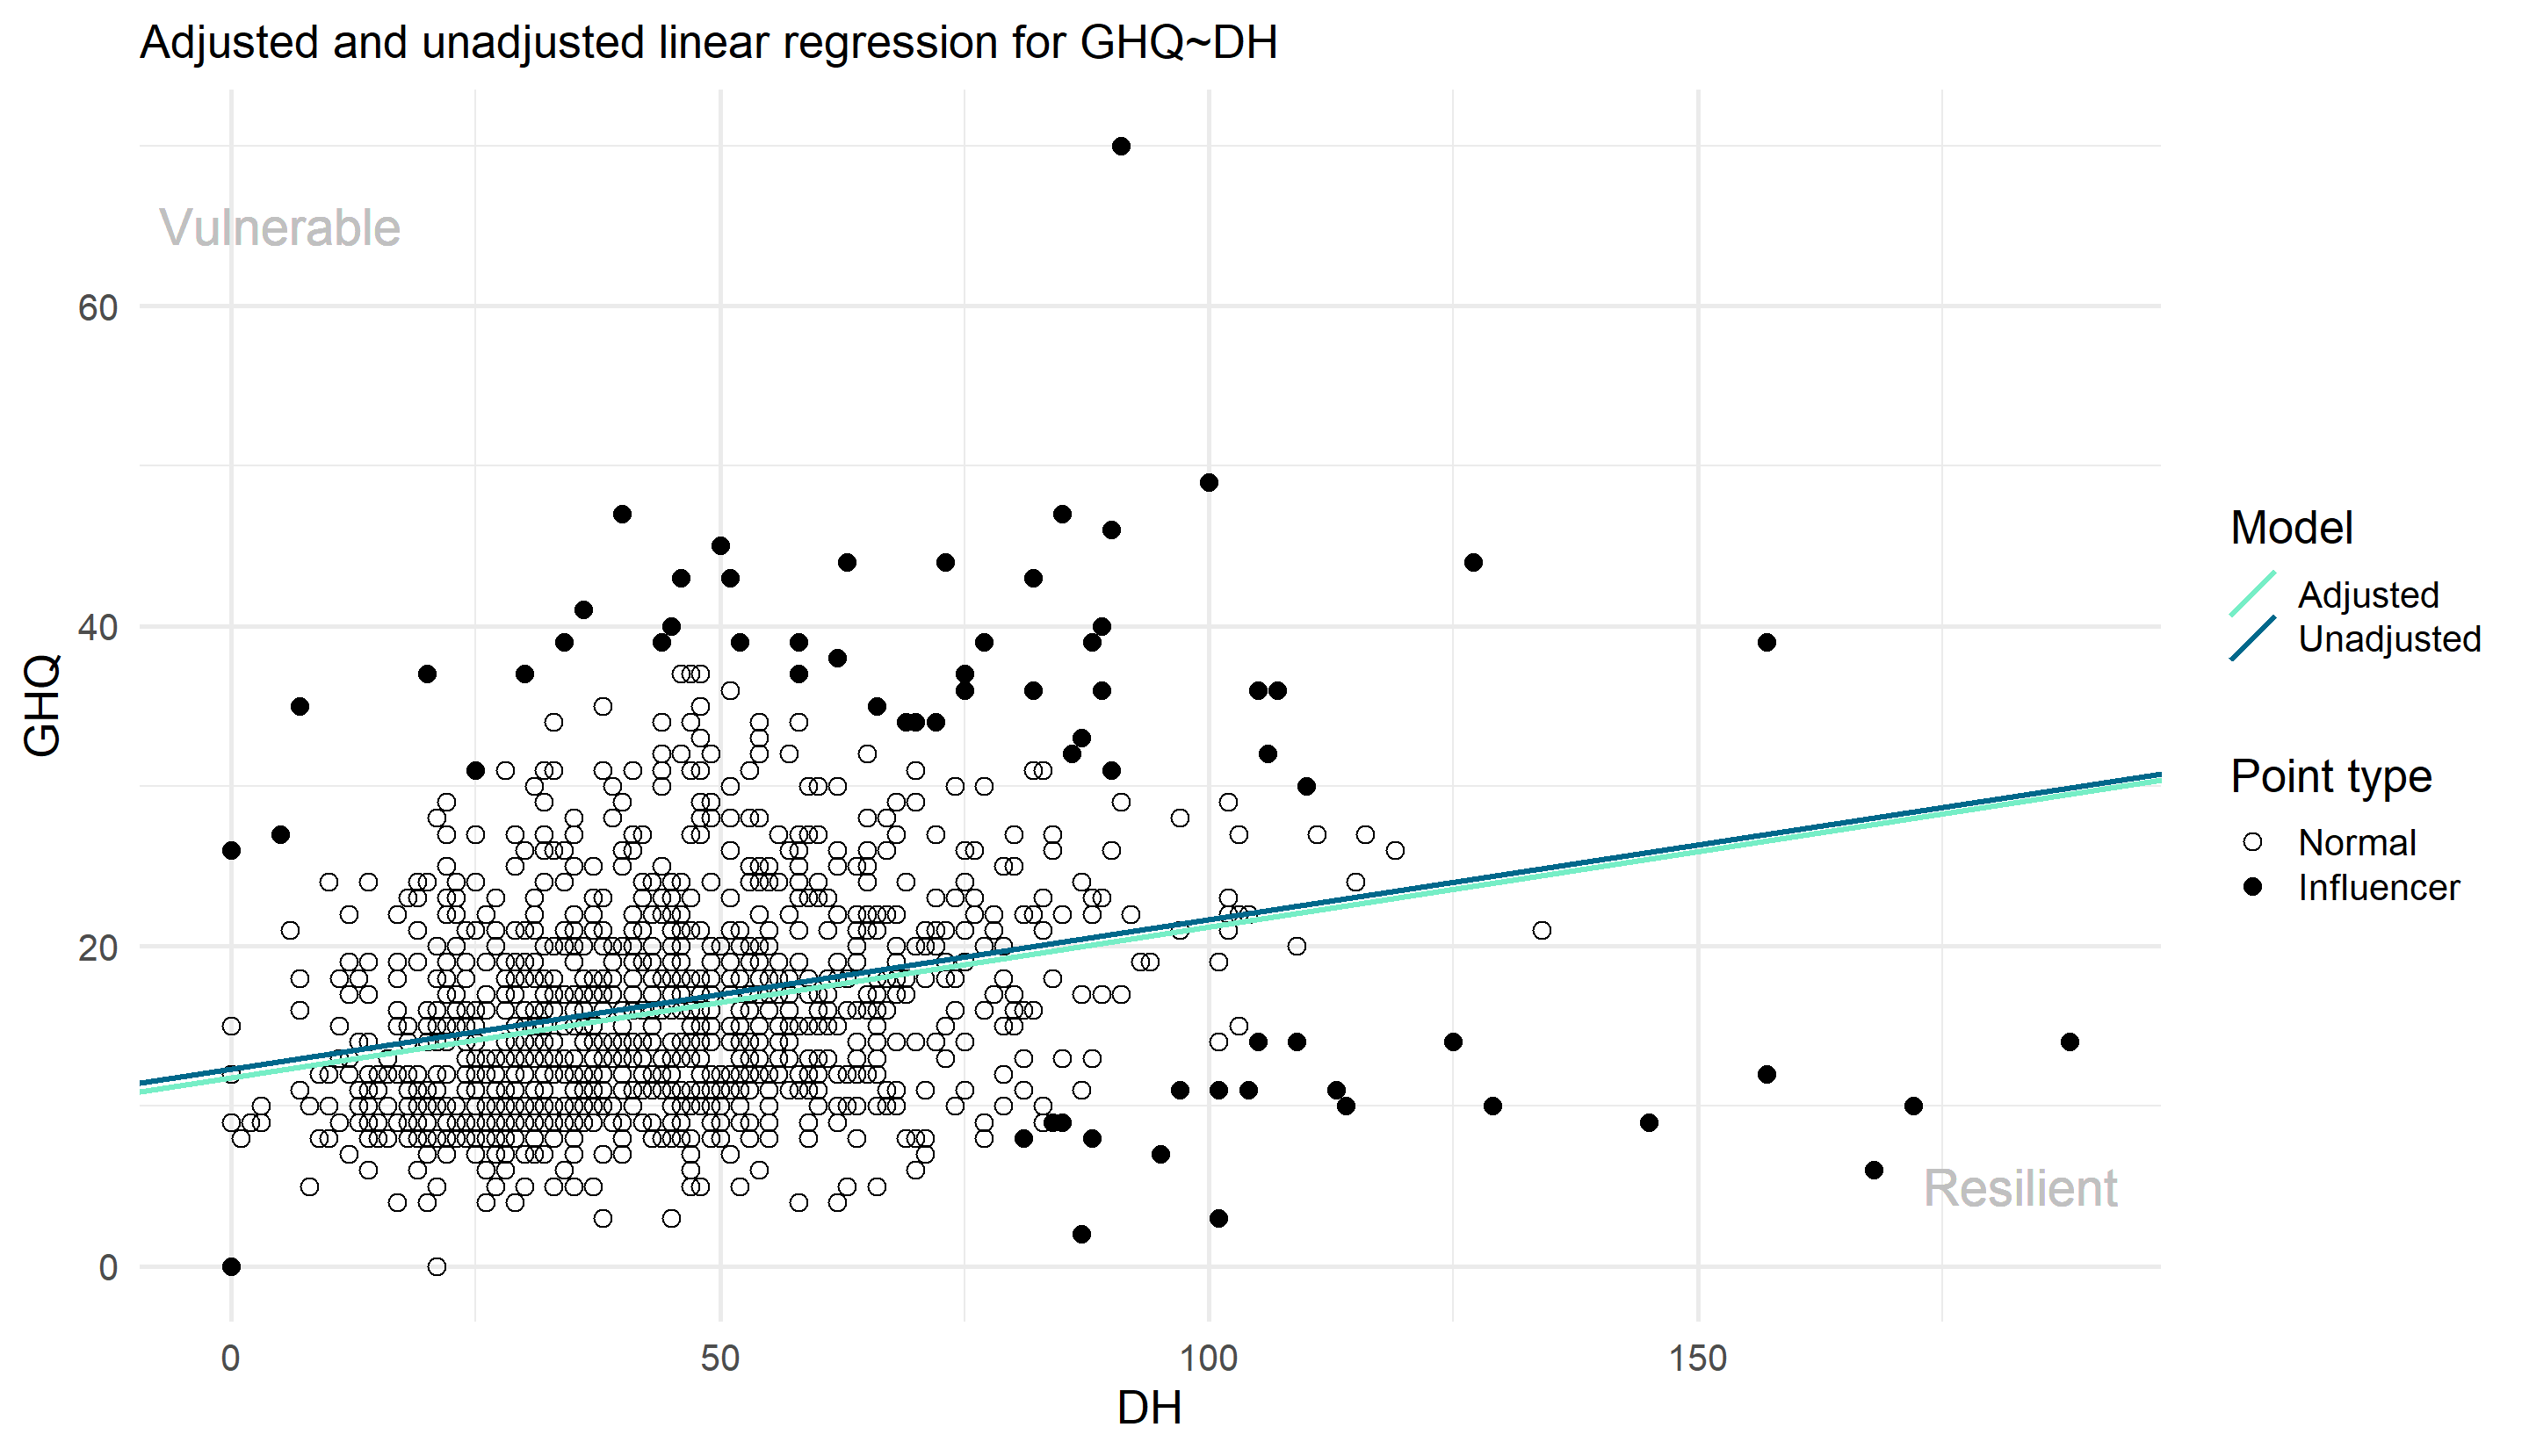
\includegraphics[width=18cm]{Pictures/LORA_Cross/DH/res.png}
    \caption{Residualization of GHQ and DH}
    \label{fig:residualization_DH}
\end{figure}

\subsubsection{Group results by method - PSS and DH}
We applied each classification method to the residuals from the adjusted linear regression for both DH and PSS and computed the resulting group memberships across all individuals each time.

\subsubsection*{Naive approach}
As shown in Table~\ref{table:size-naive-pss} and Table~\ref{table:size-naive-dh}, the naive classification method results in both cases in an extreme classification where no individuals are classified as average, all individuals are assigned either to the resilient or vulnerable group. Figures \ref{fig:classification_naive_pss} and \ref{fig:classification_naive_dh} illustrate that this method imposes a strict split at zero, without accounting for the variability or uncertainty of the residuals. Even individuals with residuals very close to zero are considered atypical. This method is therefore intended more as a baseline comparison than as a realistic classification approach.

\begin{table}[H]
\centering
\rowcolors{2}{gray!20}{white} % Gris sur une ligne sur deux
{\small
\begin{tabular}{>{\centering\arraybackslash}p{3cm}
                >{\centering\arraybackslash}p{3cm}
                >{\centering\arraybackslash}p{3cm}}
\hline
\textbf{Resilient size} & \textbf{Average size} & \textbf{Vulnerable size} \\
\hline
651& 0 & 540\\
\hline
\end{tabular}
}
\caption{Group size with the naive approach for DH}
\label{table:size-naive-dh}
\end{table}

\begin{table}[H]
\centering
\rowcolors{2}{gray!20}{white} % Gris sur une ligne sur deux
{\small
\begin{tabular}{>{\centering\arraybackslash}p{3cm}
                >{\centering\arraybackslash}p{3cm}
                >{\centering\arraybackslash}p{3cm}}
\hline
\textbf{Resilient size} & \textbf{Average size} & \textbf{Vulnerable size} \\
\hline
626& 0 & 565\\
\hline
\end{tabular}
}
\caption{Group size with the naive approach for PSS}
\label{table:size-naive-pss}
\end{table}

\begin{figure}[H]
    \centering
    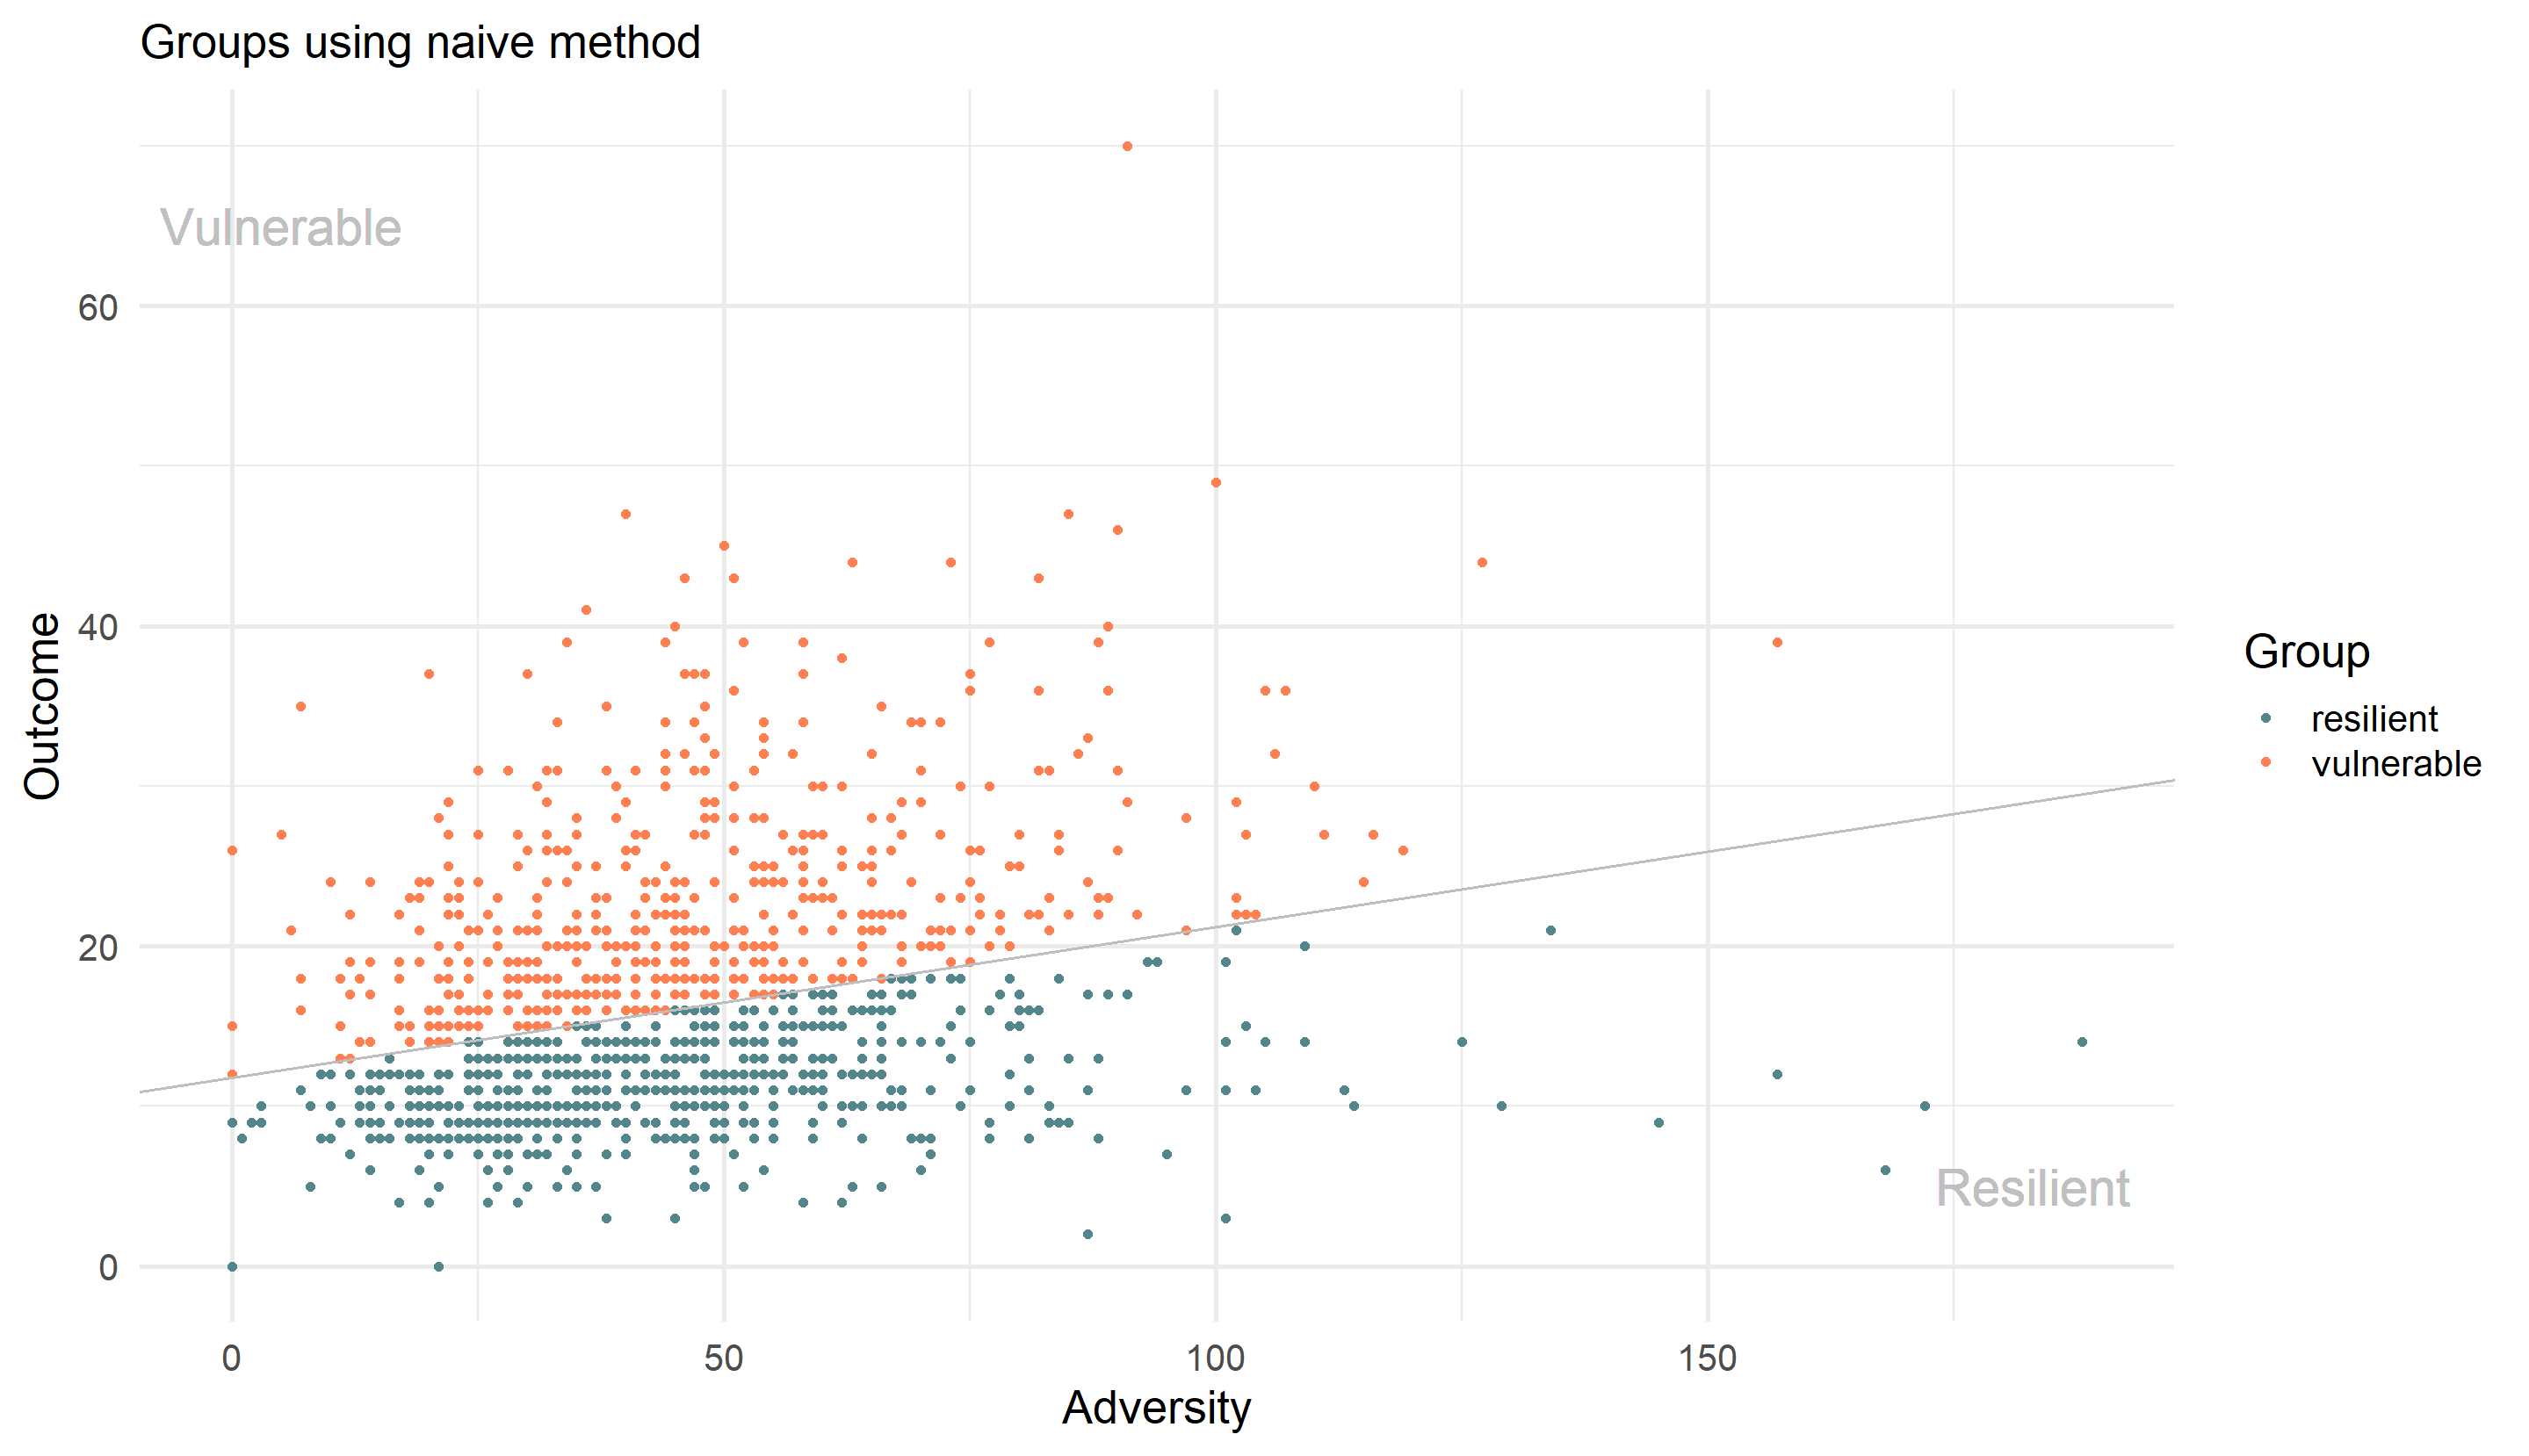
\includegraphics[width=18cm]{Pictures/LORA_Cross/DH/naive.png}
    \caption{Classification obtained with the naive approach for DH}
    \label{fig:classification_naive_dh}
\end{figure}
\begin{figure}[H]
    \centering
    
\includegraphics[width=18cm]{Pictures/LORA_Cross/PSS/naive.png}
    \caption{Classification obtained with the naive approach for PSS}
    \label{fig:classification_naive_pss}
\end{figure}

\subsubsection*{Confidence and prediction interval-based classification}
As shown in Tables~\ref{table:size-confidence_pred_dh} and ~\ref{table:size-confidence_pred_pss} and Figures~\ref{fig:conf_pred-classification_dh} and  ~\ref{fig:conf_pred-classification_pss}, prediction intervals produce wider intervals and thus larger average groups compared to confidence intervals. In both cases, the 3 values tested for prediction intervals ($50,60$ and $75$\%) resulted in a dominant average group, but not the two confidence intervals tested ($99$ and $90$\%), which resulted in a bigger resilient group. As expected, decreasing the confidence or prediction level (i.e., using a smaller \(1-\alpha \)) results in narrower intervals and, consequently, smaller average groups. \\
\\
An important distinction in our results is that confidence intervals exhibit much greater variation in width across levels of adversity than prediction intervals. This arises because, in both models, the leverage term \( x_0^\top (\mathbf{X}^\top \mathbf{X})^{-1} x_0 \) remains very small in both cases, leading to a wider range of variation for the standard error for the confidence intervals than the prediction intervals:\\
\\
For the Daily Hassles (DH) model, the standard error for the mean prediction varies between:
\[
0.0008 \leq \text{SE}_{\text{mean}}(x_0) \leq 0.020,
\]
while the standard error for the prediction interval remains nearly constant:
\[
1.000 \leq \text{SE}_{\text{pred}}(x_0) \leq 1.009.
\]
Similarly, for the Perceived Stress Scale (PSS) model:
\[
0.0008 \leq \text{SE}_{\text{mean}}(x_0) \leq 0.0115,
\]
compared to:
\[
1.000 \leq \text{SE}_{\text{pred}}(x_0) \leq 1.006.
\]
These results show that prediction intervals appear almost uniform across the range of adversity, while confidence intervals are more sensitive to an individual’s adversity level.



\begin{table}[H]
\centering
\rowcolors{2}{gray!20}{white} % Gris sur une ligne sur deux
{\small
\begin{tabular}{>{\centering\arraybackslash}p{5cm}
                >{\centering\arraybackslash}p{3cm}
                >{\centering\arraybackslash}p{3cm}
                >{\centering\arraybackslash}p{3cm}}
\hline
\textbf{Detail}&\textbf{Resilient size} & \textbf{Average size} & \textbf{Vulnerable size} \\
\hline
Prediction interval 75\% &125&870&196\\
Prediction interval 60\% & 252&688&251\\
Prediction interval 50\% & 342&550&299\\
Confidence interval 99\% &612& 89&490\\
Confidence interval 90\%&620&71&500\\
\hline
\end{tabular}
}
\caption{Group size with the confidence and prediction intervals approach for DH}
\label{table:size-confidence_pred_dh}
\end{table}
\begin{figure}[H]
    \centering
    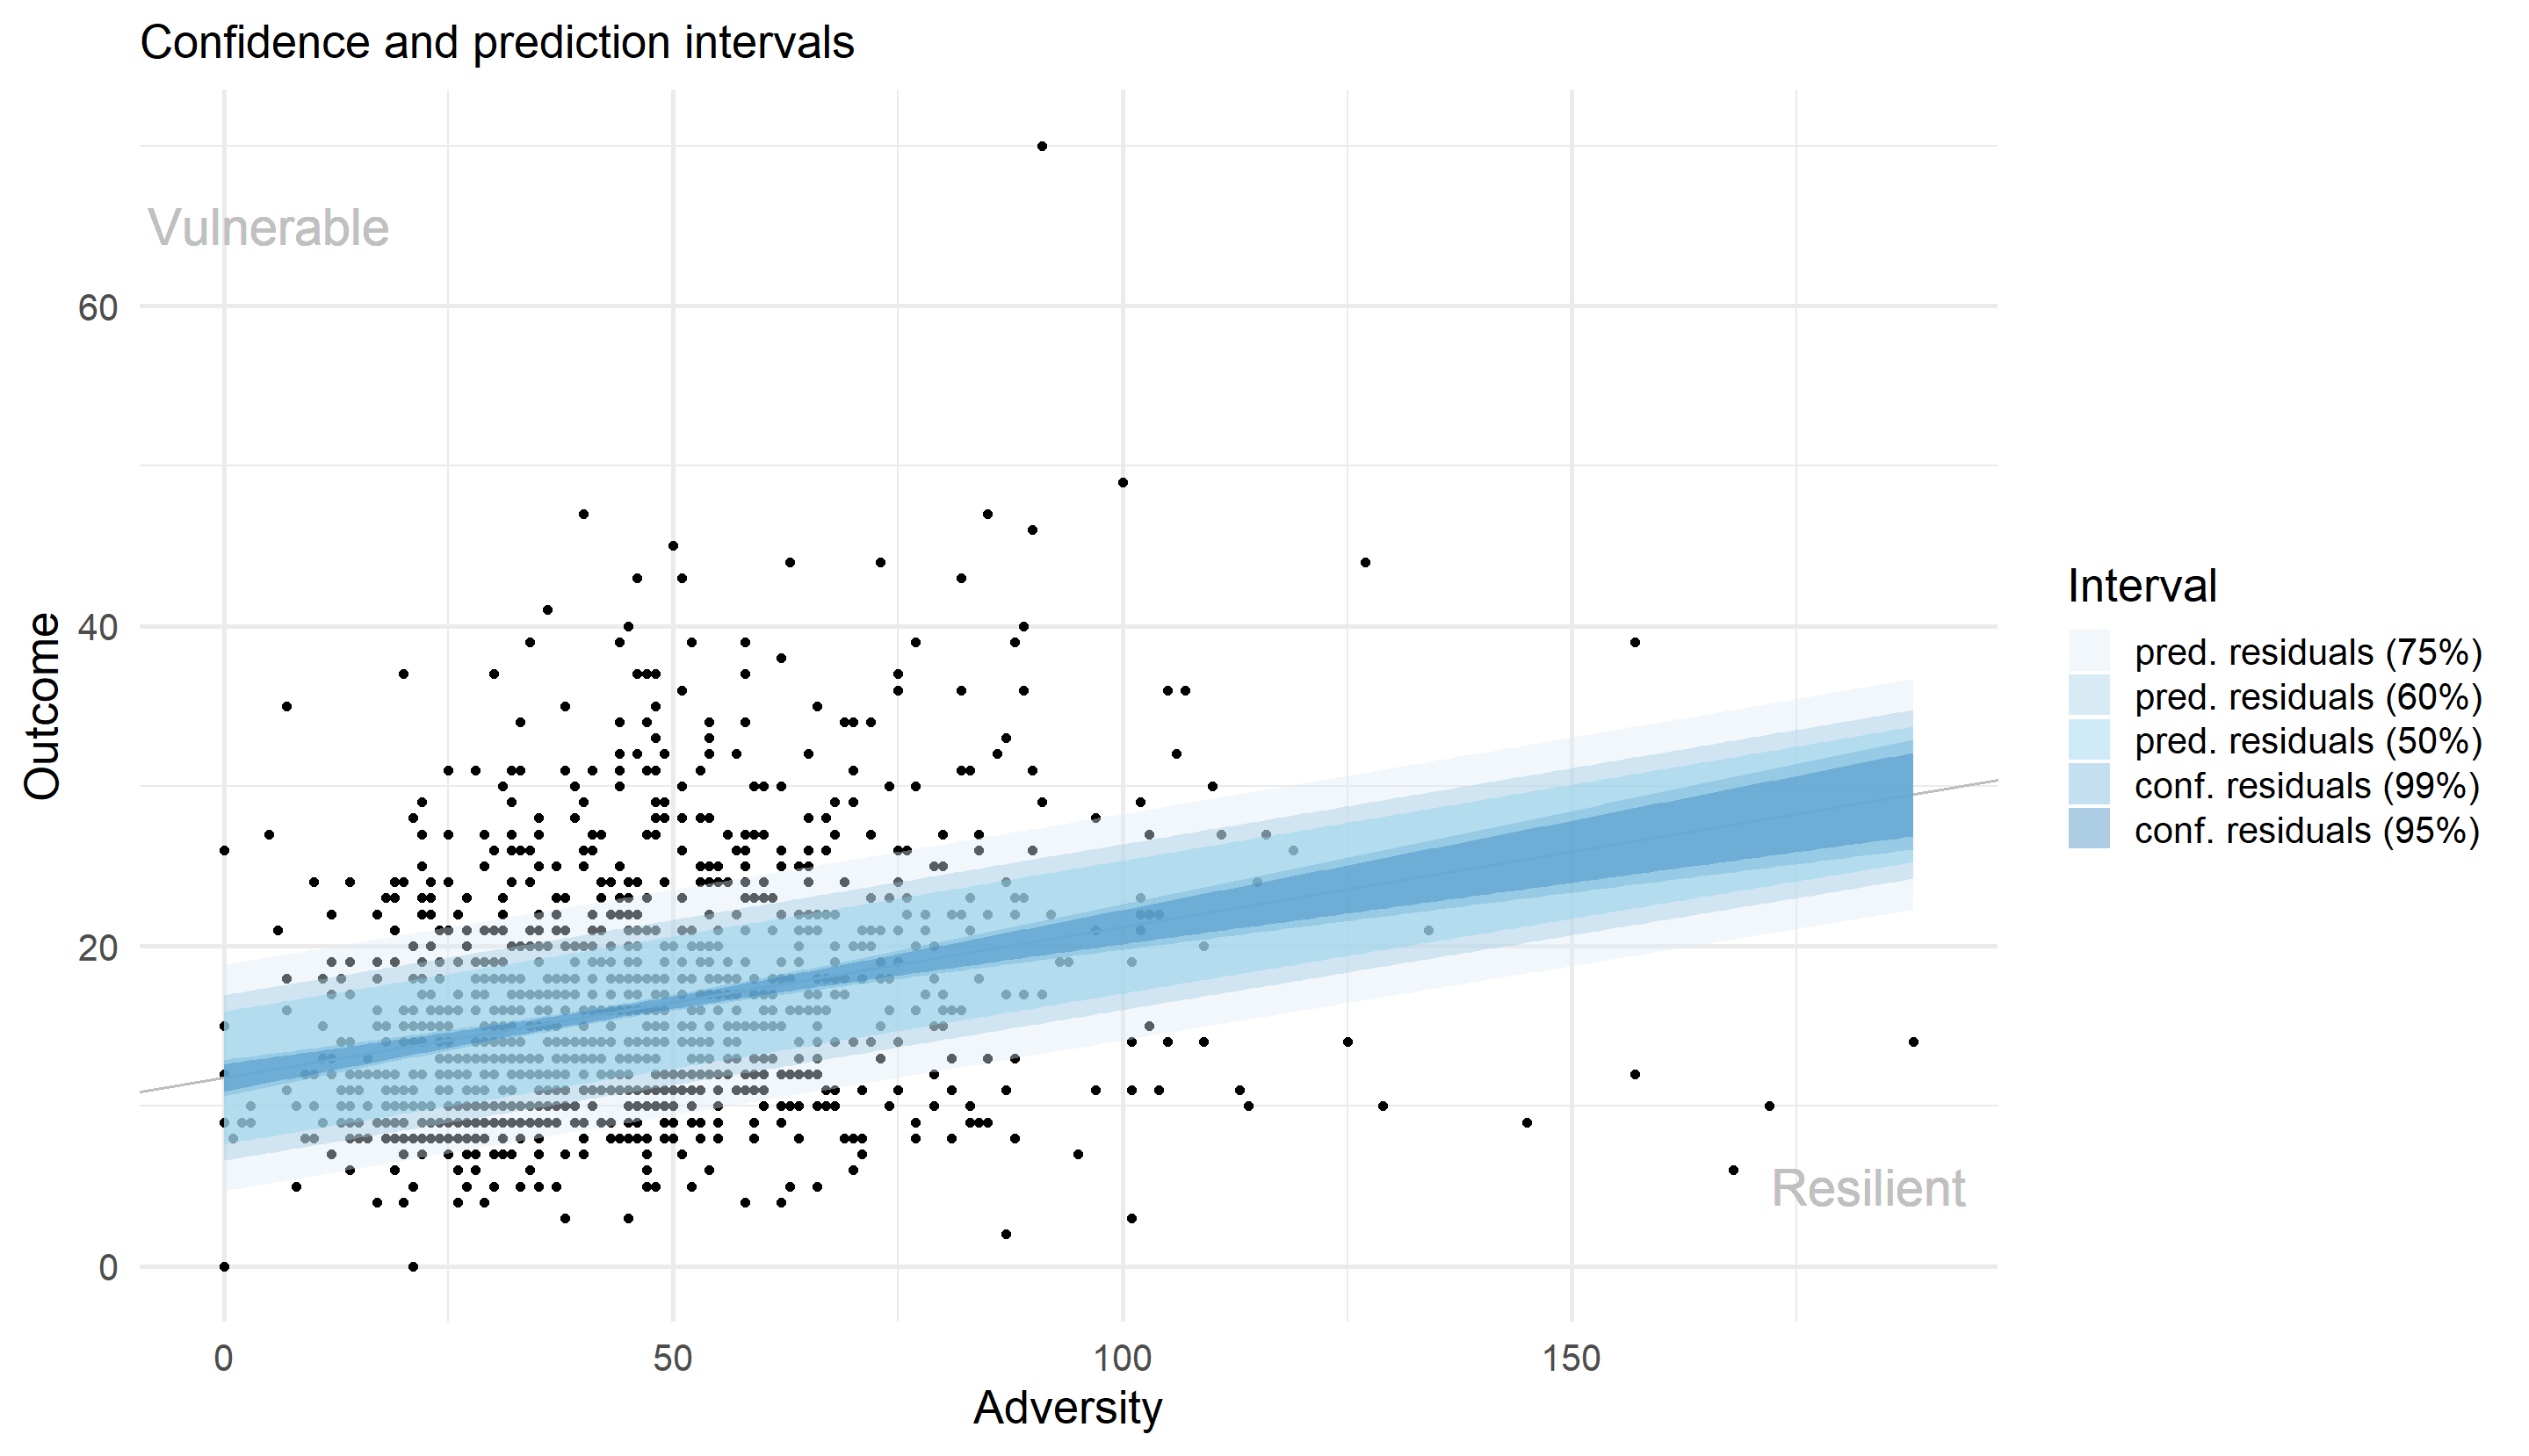
\includegraphics[width=18cm]{Pictures/LORA_Cross/DH/confpred.png}
    \caption{Classification obtained with the confidence and prediction intervals approach for DH}
    \label{fig:conf_pred-classification_dh}
\end{figure}

\begin{table}[H]
\centering
\rowcolors{2}{gray!20}{white} % Gris sur une ligne sur deux
{\small
\begin{tabular}{>{\centering\arraybackslash}p{5cm}
                >{\centering\arraybackslash}p{3cm}
                >{\centering\arraybackslash}p{3cm}
                >{\centering\arraybackslash}p{3cm}}
\hline
\textbf{Detail}&\textbf{Resilient size} & \textbf{Average size} & \textbf{Vulnerable size} \\
\hline
Prediction interval 75\% &137&850&204\\
Prediction interval 60\% & 252&665&274\\
Prediction interval 50\% & 317&554&320\\
Confidence interval 99\% &576& 101&514\\
Confidence interval 90\%&594&74&523\\
\hline
\end{tabular}
}
\caption{Group size with the confidence and prediction intervals approach for PSS}
\label{table:size-confidence_pred_pss}
\end{table}
\begin{figure}[H]
    \centering
    
\includegraphics[width=18cm]{Pictures/LORA_Cross/PSS/confpred.png}
    \caption{Classification obtained with the confidence and prediction intervals approach for PSS}
    \label{fig:conf_pred-classification_pss}
\end{figure}

\subsubsection*{Credibility interval-based classification}
As shown in Figure~\ref{fig:credibility-classification-dh} and Figure~\ref{fig:credibility-classification-pss} and Tables~\ref{table:size-credibility-dh} and \ref{table:size-credibility-pss}, credibility intervals tend to be very narrow, resulting in small average groups, even when using wide intervals such as the 99.9\% credibility level. In practice, the class size produced by credibility intervals resembles those obtained from confidence intervals of the same level.\\
\\
As with confidence intervals, the width of credibility intervals varies with the level of adversity, since they reflect posterior uncertainty around the expected outcome for each individual.

\begin{table}[H]
\centering
\rowcolors{2}{gray!20}{white} % Gris sur une ligne sur deux
{\small
\begin{tabular}{>{\centering\arraybackslash}p{4cm}
                >{\centering\arraybackslash}p{3cm}
                >{\centering\arraybackslash}p{3cm}
                >{\centering\arraybackslash}p{3cm}}
\hline
\textbf{Detail}&\textbf{Resilient size} & \textbf{Average size} & \textbf{Vulnerable size} \\
\hline
Credibility interval 99.9\% & 629& 118& 444\\
Credibility interval 99\% & 635& 102& 454\\
Credibility interval 95\% & 654& 70&467\\
Credibility interval 90\% & 655& 64& 472\\
Credibility interval 75\% & 665& 43& 483\\
Credibility interval 50\% & 683& 20& 488\\
\hline
\end{tabular}
}
\caption{Group size with the credibility intervals approach for DH}
\label{table:size-credibility-dh}
\end{table}
\begin{figure}[H]
    \centering
    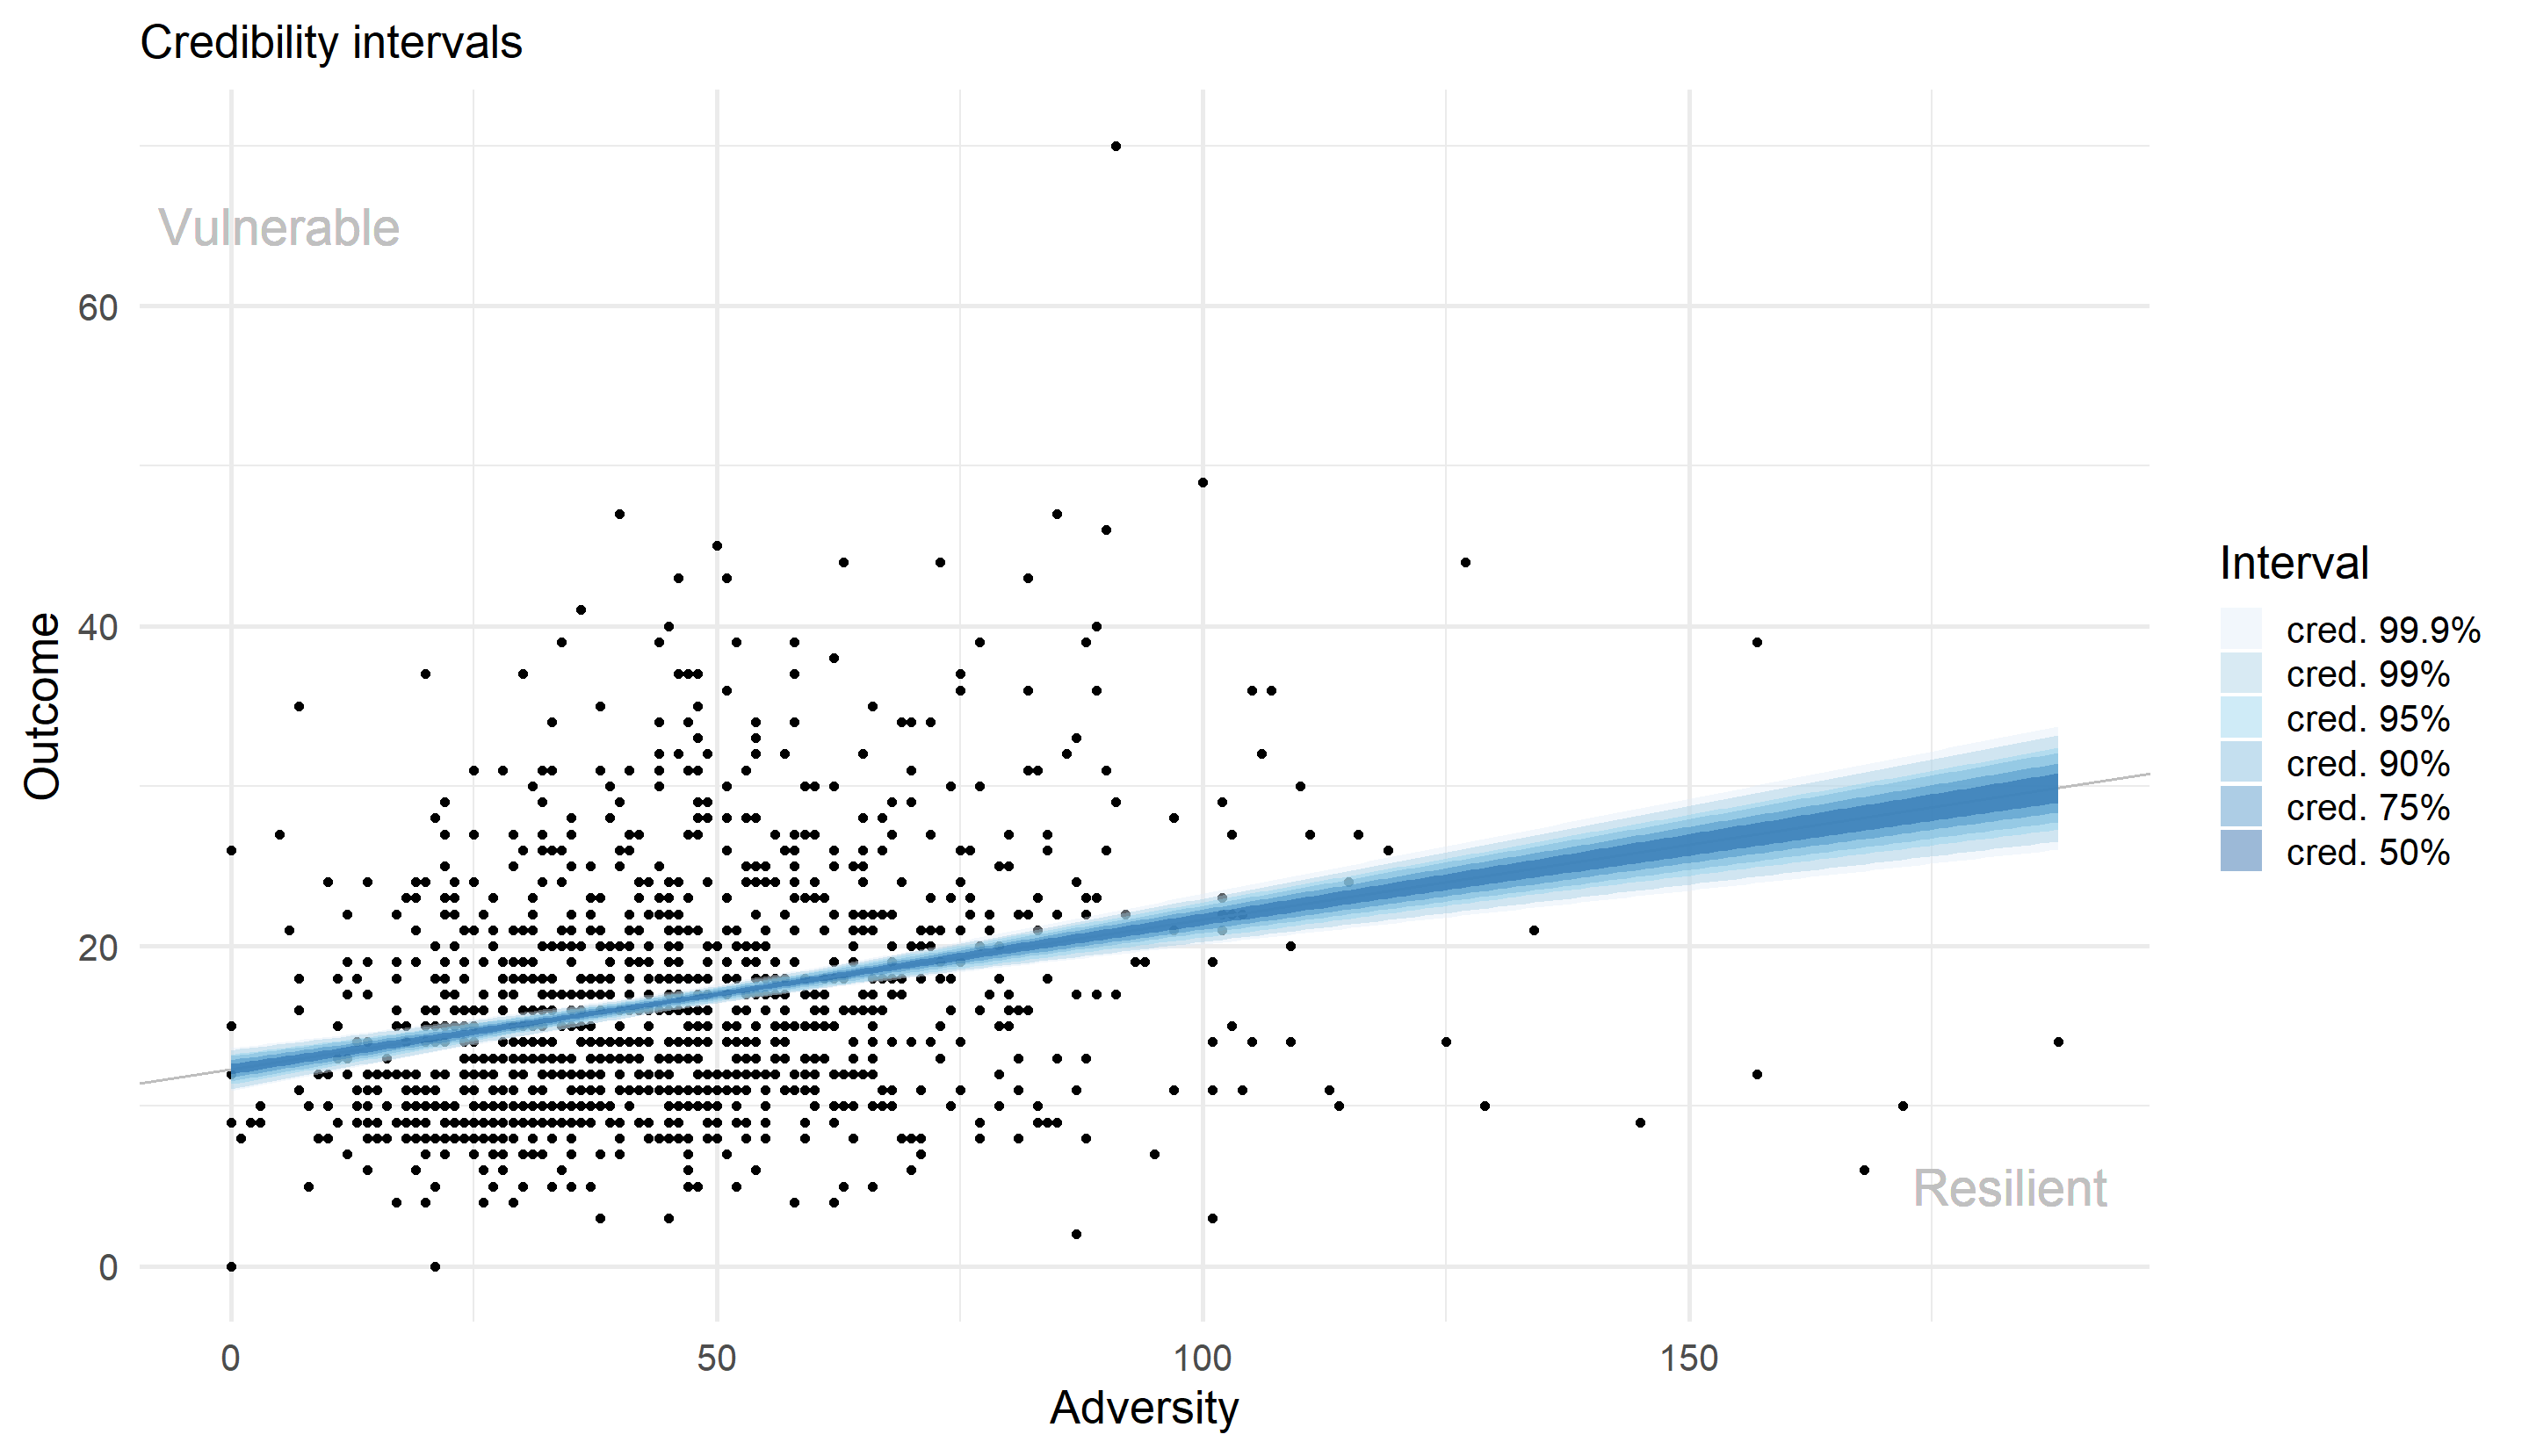
\includegraphics[width=18cm]{Pictures/LORA_Cross/DH/credibility.png}
    \caption{Classification obtained with the credibility intervals approach for DH}
    \label{fig:credibility-classification-dh}
\end{figure}

\begin{table}[H]
\centering
\rowcolors{2}{gray!20}{white} % Gris sur une ligne sur deux
{\small
\begin{tabular}{>{\centering\arraybackslash}p{4cm}
                >{\centering\arraybackslash}p{3cm}
                >{\centering\arraybackslash}p{3cm}
                >{\centering\arraybackslash}p{3cm}}
\hline
\textbf{Detail}&\textbf{Resilient size} & \textbf{Average size} & \textbf{Vulnerable size} \\
\hline
Credibility interval 99.9\% & 599& 131& 461\\
Credibility interval 99\% & 610& 109& 472\\
Credibility interval 95\% & 622& 83&486\\
Credibility interval 90\% & 633& 66& 492\\
Credibility interval 75\% & 643& 45& 503\\
Credibility interval 50\% & 652& 23& 516\\
\hline
\end{tabular}
}
\caption{Group size with the credibility intervals approach for PSS}
\label{table:size-credibility-pss}
\end{table}
\begin{figure}[H]
    \centering
    
\includegraphics[width=18cm]{Pictures/LORA_Cross/PSS/credibility.png}
    \caption{Classification obtained with the credibility intervals approach for PSS}
    \label{fig:credibility-classification-pss}
\end{figure}

\subsubsection*{Quantile-based thresholds}
In this approach, quantile thresholds were computed using only individuals identified as not overly influential, but the resulting classifications were applied to the full sample. As shown in Tables~\ref{table:size-quantiles-dh} and \ref{table:size-quantiles-pss}, the quantile-based method yields approximately symmetrical group sizes by construction, with typically fewer than fifty individuals separating the resilient and vulnerable groups.\\
\\
The size of the average group depends directly on the chosen quantile level \( n\% \). For example, setting \( n = 5\% \) to \( 30\% \) results in a dominant average group. However, beyond \(n=35\% \), the average group becomes smaller than the two atypical groups.\\
\\
This method is particularly useful when a predefined proportion of the population is intended to be classified as atypical or normative, offering direct control over group sizes.

\begin{table}[H]
\centering
\rowcolors{2}{gray!20}{white} % Gris sur une ligne sur deux
{\small
\begin{tabular}{>{\centering\arraybackslash}p{4cm}
                >{\centering\arraybackslash}p{3cm}
                >{\centering\arraybackslash}p{3cm}
                >{\centering\arraybackslash}p{3cm}}
\hline
\textbf{Detail}&\textbf{Resilient size} & \textbf{Average size} & \textbf{Vulnerable size} \\
\hline
5\% & 79& 1013& 99\\
10\% & 137& 897& 157\\
15\% & 193& 784& 214\\
20\% &  249& 672& 270\\
25\% & 307& 556& 328\\
30\% & 361& 448& 382\\
35\% & 417& 336& 438\\
\hline
\end{tabular}
}
\caption{Group size with the quantile approach for DH}
\label{table:size-quantiles-dh}
\end{table}

\begin{table}[H]
\centering
\rowcolors{2}{gray!20}{white} % Gris sur une ligne sur deux
{\small
\begin{tabular}{>{\centering\arraybackslash}p{4cm}
                >{\centering\arraybackslash}p{3cm}
                >{\centering\arraybackslash}p{3cm}
                >{\centering\arraybackslash}p{3cm}}
\hline
\textbf{Detail}&\textbf{Resilient size} & \textbf{Average size} & \textbf{Vulnerable size} \\
\hline
5\% & 73& 1010& 108\\
10\% & 131& 893& 167\\
15\% & 187& 780& 224\\
20\% &  252& 660& 279\\
25\% & 301& 556& 334\\
30\% & 354& 444& 393\\
35\% & 418& 325& 448\\
\hline
\end{tabular}
}
\caption{Group size with the quantile approach for PSS}
\label{table:size-quantiles-pss}
\end{table}
\subsubsection*{Standard deviation-based thresholds with adversity levels}
The standard deviation-based approach was applied using the following cutoffs: 0-13,14-26 and 27-40 for PSS and 0-75, 76-150, and 151-226 for DH.\\
\\
Like for the quantiles, the individuals marked as not overly influential were not used to compute the standard deviation of each bin, but the classification was applied to all individuals. Since all individuals in the 151-226 bin for DH were considered overly influential, the standard deviation of this bin is set to 0, and all individuals are non-average.\\
\\
As shown in Tables~\ref{table:size-sd-dh} and \ref{table:size-sd-pss} and Figures~\ref{fig:sd-classification-dh} and \ref{fig:sd-classification-pss}, this approach can produce either very large or very small average groups depending on the chosen threshold. For example, using a threshold of 0.5 SD around the prediction results in approximately 16\% of individuals being classified as average for DH and 18\% for PSS. In contrast, the 2SD threshold yields an average group comprising around 98\% of the sample for DH and 99\% for PSS.\\
\\
This method also allows the width of the average band to vary across adversity levels, as the standard deviation is computed within each category. This provides an additional layer of flexibility, as the classification adapts to the variability within each adversity group.

\begin{table}[H]
\centering
\rowcolors{2}{gray!20}{white} % Gris sur une ligne sur deux
{\small
\begin{tabular}{>{\centering\arraybackslash}p{4cm}
                >{\centering\arraybackslash}p{3cm}
                >{\centering\arraybackslash}p{3cm}
                >{\centering\arraybackslash}p{3cm}}
\hline
\textbf{Detail (multiplication)}&\textbf{Resilient size} & \textbf{Average size} & \textbf{Vulnerable size} \\
\hline
2SD &  3& 1174& 14\\
1SD &  175& 796& 220\\
0.5SD &  549&197&445\\
\hline
\end{tabular}
}
\caption{Group size with the standard deviation approach for DH}
\label{table:size-sd-dh}
\end{table}
\begin{figure}[H]
    \centering
    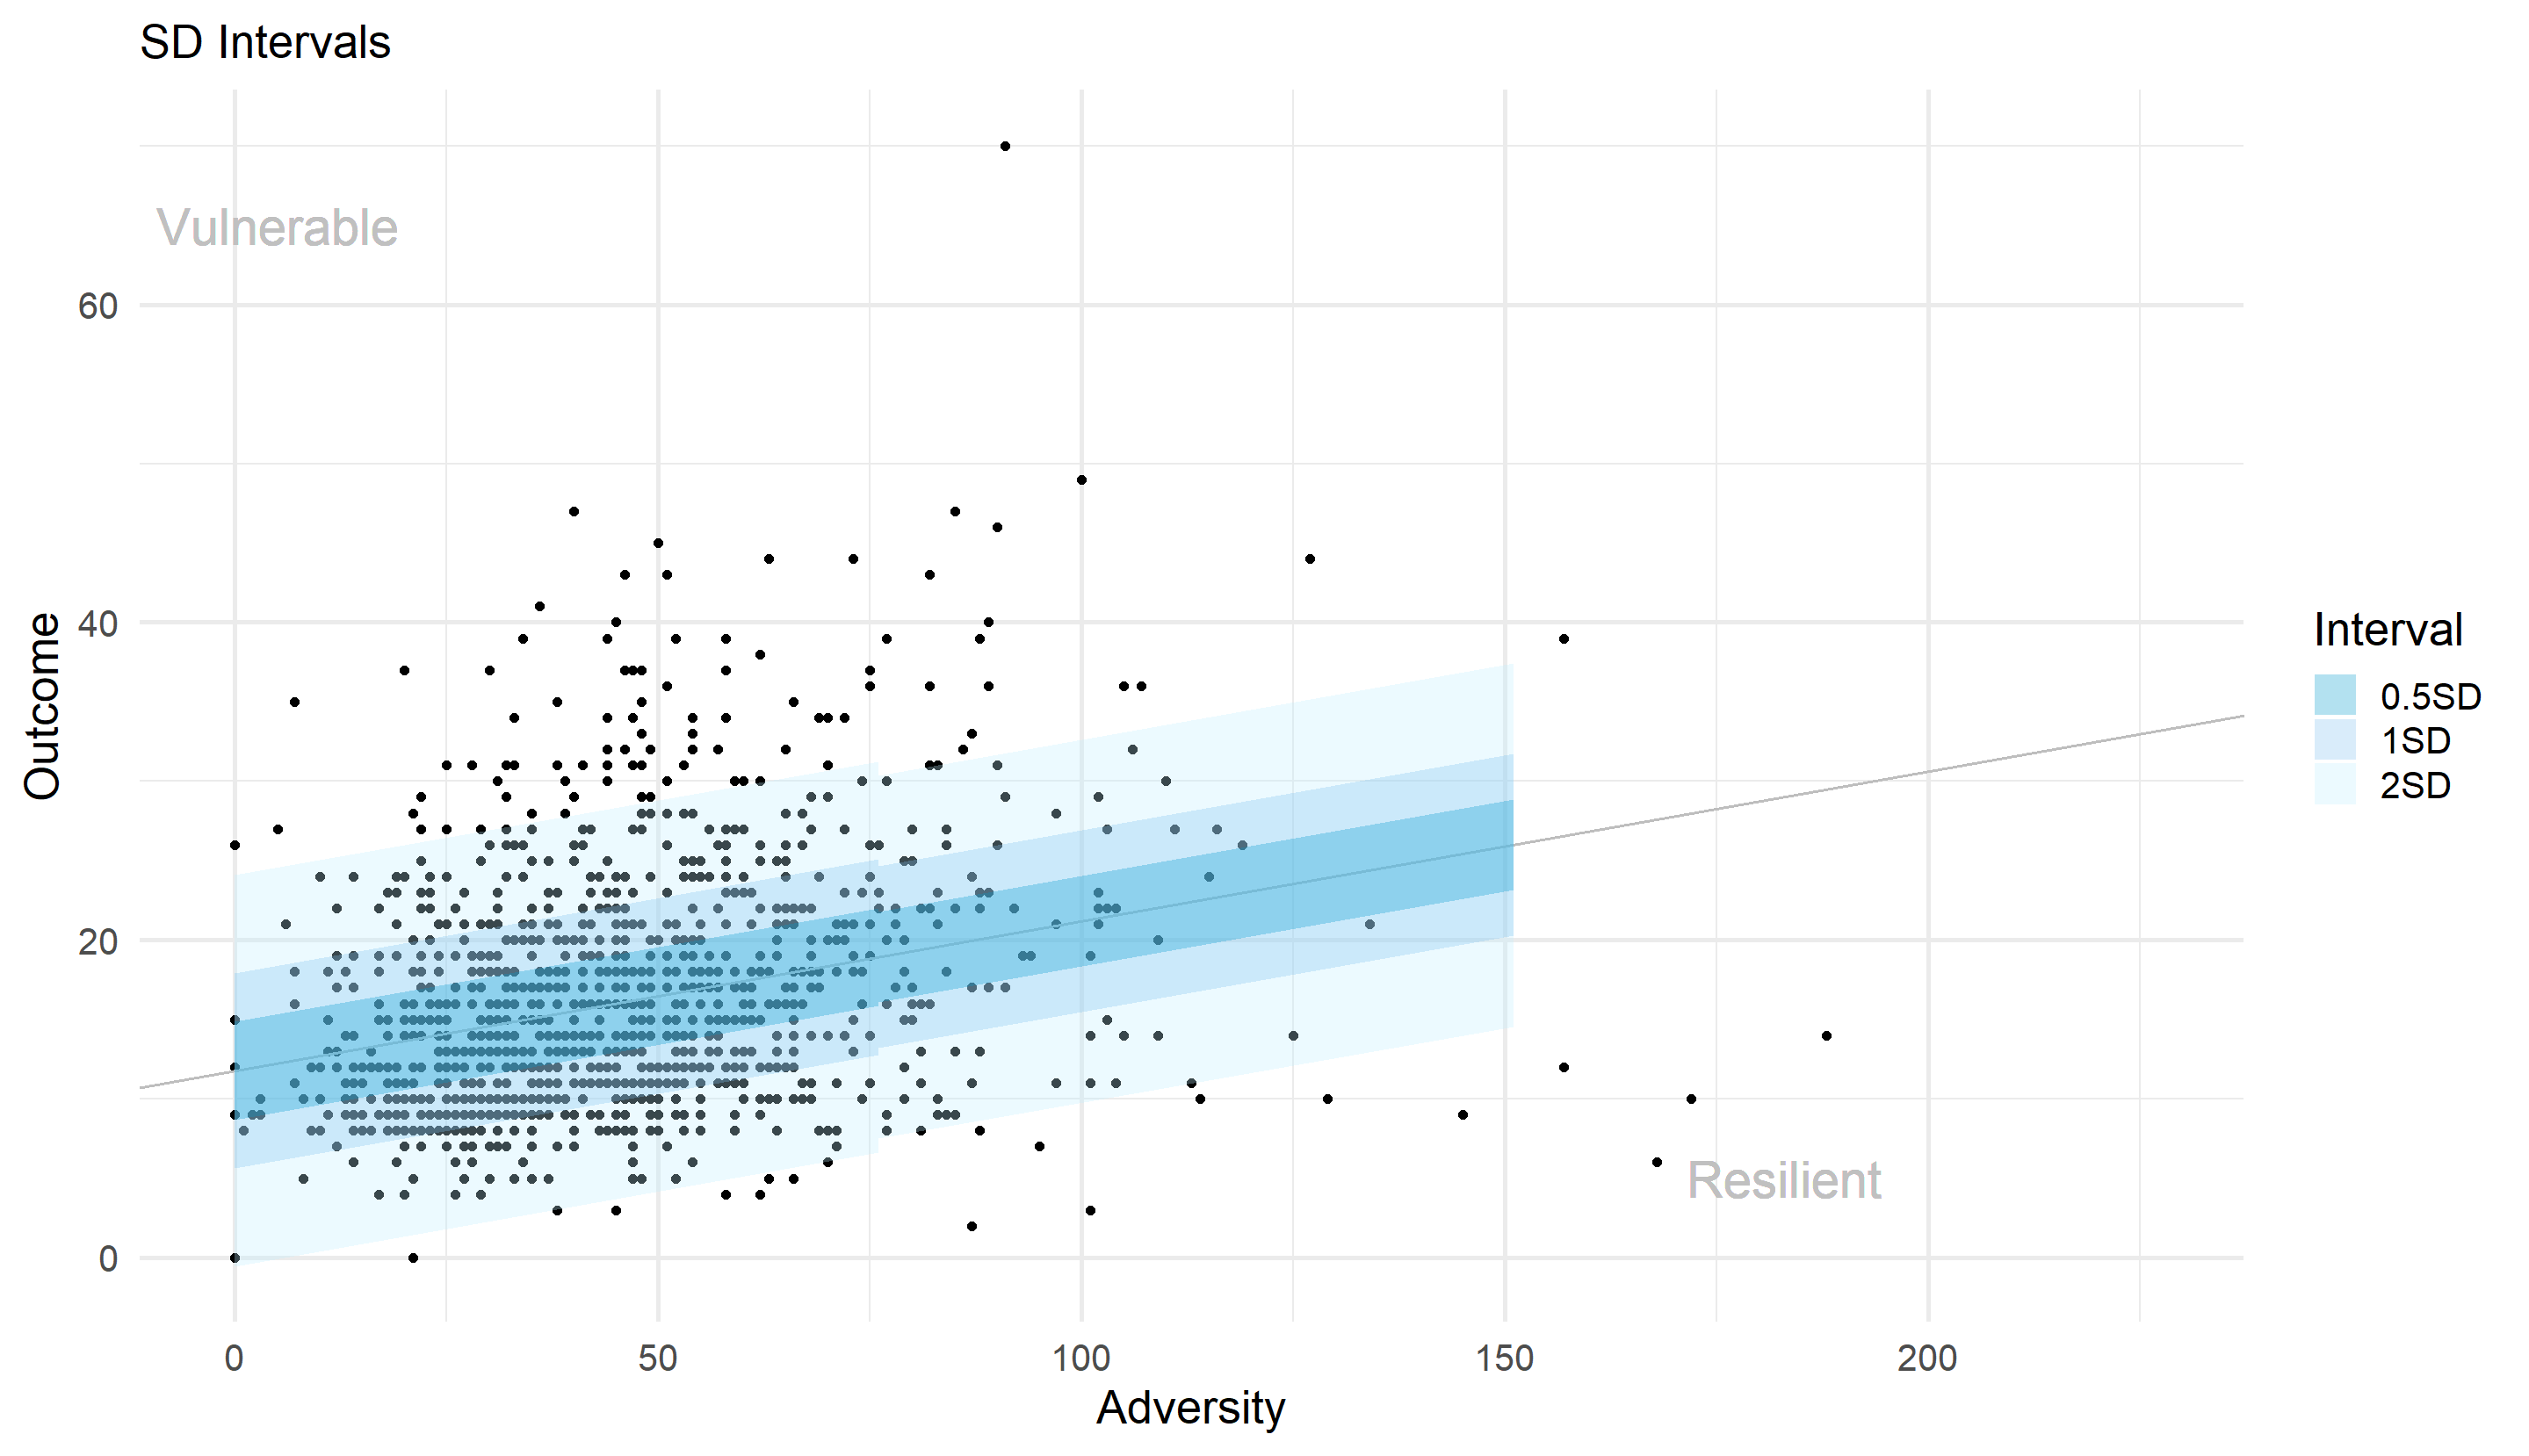
\includegraphics[width=18cm]{Pictures/LORA_Cross/DH/sd.png}
    \caption{Classification obtained with the standard deviation approach for DH}
    \label{fig:sd-classification-dh}
\end{figure}

\begin{table}[H]
\centering
\rowcolors{2}{gray!20}{white} % Gris sur une ligne sur deux
{\small
\begin{tabular}{>{\centering\arraybackslash}p{4cm}
                >{\centering\arraybackslash}p{3cm}
                >{\centering\arraybackslash}p{3cm}
                >{\centering\arraybackslash}p{3cm}}
\hline
\textbf{Detail (multiplication)}&\textbf{Resilient size} & \textbf{Average size} & \textbf{Vulnerable size} \\
\hline
2SD &  1& 1179& 11\\
1SD &  192& 762& 237\\
0.5SD &  524&219&448\\
\hline
\end{tabular}
}
\caption{Group size with the standard deviation approach for PSS}
\label{table:size-sd-pss}
\end{table}
\begin{figure}[H]
    \centering
    
\includegraphics[width=18cm]{Pictures/LORA_Cross/PSS/sd.png}
    \caption{Classification obtained with the standard deviation approach for PSS}
    \label{fig:sd-classification-pss}
\end{figure}

\subsubsection*{K-means classification}
Again, for this approach, we only used the individuals identified as not overly influential to construct the k-means clusters. The remaining individuals were assigned to the cluster whose centre they were closest to.\\
\\
As shown in Tables~\ref{table:size-kmeans-dh} and \ref{table:size-kmeans-pss}, the classification produced by the k-means-based approach is not symmetrical: the resilient group is notably bigger than the other two groups for DH and in the case of PSS, although the average group is the biggest, the resilient group is notably bigger than the vulnerable group and closer in size to the average group. This reflects the data-driven nature of the method, which does not impose balanced group sizes or fixed thresholds, but instead discovers clusters based on the structure of the residual distribution.\\
\\
An advantage of this approach, as shown in Figures~\ref{fig:kmeans-classification-dh} and \ref{fig:kmeans-classification-pss}, is that, despite relying solely on the data, it still identifies a central group composed of individuals with small positive and small negative residuals, corresponding well to the notion of an average or normative response. In contrast, unsupervised methods could, in principle, produce less interpretable groupings (e.g., two clusters of positive residuals and one of negative), but this was not the case here. However, the fact that the resilient and vulnerable groups can be very different in size and that the average group is not dominant in the case of DH highlights the method’s sensitivity to distributional shape. 

\begin{table}[H]
\centering
\rowcolors{2}{gray!20}{white} % Gris sur une ligne sur deux
{\small
\begin{tabular}{>{\centering\arraybackslash}p{3cm}
                >{\centering\arraybackslash}p{3cm}
                >{\centering\arraybackslash}p{3cm}}
\hline
\textbf{Resilient size} & \textbf{Average size} & \textbf{Vulnerable size} \\
\hline
537& 439& 215\\
\hline
\end{tabular}
}
\caption{Group size with the k-means approach for DH}
\label{table:size-kmeans-dh}
\end{table}
\begin{figure}[H]
    \centering
    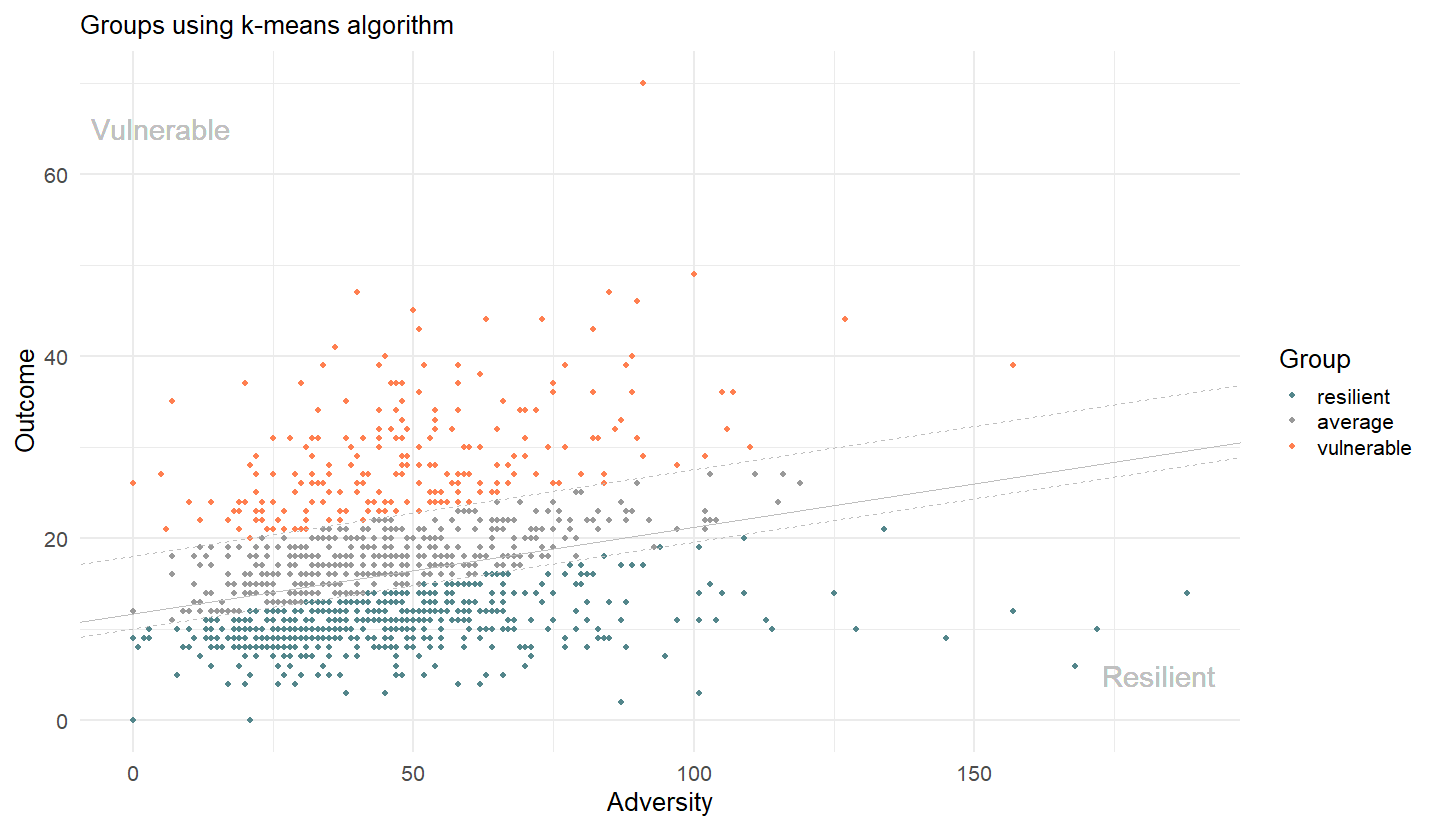
\includegraphics[width=18cm]{Pictures/LORA_Cross/DH/k-means.png}
    \caption{Classification obtained with the k-means method for DH}
    \label{fig:kmeans-classification-dh}
\end{figure}

\begin{table}[H]
\centering
\rowcolors{2}{gray!20}{white} % Gris sur une ligne sur deux
{\small
\begin{tabular}{>{\centering\arraybackslash}p{3cm}
                >{\centering\arraybackslash}p{3cm}
                >{\centering\arraybackslash}p{3cm}}
\hline
\textbf{Resilient size} & \textbf{Average size} & \textbf{Vulnerable size} \\
\hline
437& 475& 279\\
\hline
\end{tabular}
}
\caption{Group size with the k-means approach for PSS}
\label{table:size-kmeans-pss}
\end{table}
\begin{figure}[H]
    \centering
    
\includegraphics[width=18cm]{Pictures/LORA_Cross/PSS/k-means.png}
    \caption{Classification obtained with the k-means method for PSS}
    \label{fig:kmeans-classification-pss}
\end{figure}



\subsubsection{Evaluation of predictive relevance}
To assess whether certain classification methods are more suitable for resilience research, we evaluated their usability to build a performant training dataset for supervised prediction tasks. Specifically, we compared how well each grouping obtained supports the training of a random forest classifier to predict group membership using a set of covariates.\\
\\
We used the multiple predictors available in the LORA dataset (listed in Table~\ref{table:variables_lora}). For BFI, CDRISK, CERQ, CTQ, FSOZU, GPASS, GSE, IELC, LE and LOTR, we used the sum scores. For the COPE variable, we used the sum score of the 14 subscales. The other variables were used as is. We retained only individuals with non-missing gender and age information, and we excluded individuals with more than 30\% of missing data across the selected predictors. This resulted in a final sample of \( N = 1{,}188 \) individuals, identical for both the $GHQ\sim DH$ and $GHQ\sim PSS$  models. Missing values were imputed using the \texttt{missForest} package (version~1.5).\\
\\
When building classifiers, to reduce multicollinearity, we applied variance inflation factor (VIF) filtering using the \texttt{car} package (version~3.1-3), with a threshold of 5. We trained random forest classifiers using the \texttt{randomForest} package (version~4.7-1.2) with $500$ trees and $\lfloor\sqrt{\text{\#predictors after VIF}} \rfloor$ variables randomly sampled as candidates at each splot. Model performance was evaluated using \( k \)-fold cross-validation implemented via the \texttt{caret} package (version~7.0-1), we used $10$ folds.

\begin{table}[H]
\centering
\rowcolors{2}{gray!20}{white}
{\small
\begin{tabular}{>{\centering\arraybackslash}p{3.5cm}
>{\centering\arraybackslash}p{12cm}}
\hline
\textbf{Name} & \textbf{Description}\\
\hline
Age & Age\\
Gender & Gender\\
Income  & Income of the individual\\
Employment status  & Employment status of the individual (binary)\\
BFI  & Big Five Inventory \\
CDRISK  & Connor-Davidson Resilience Scale\\
CERQ  & Cognitive Emotion Regulation Questionnaire\\
COPE  & Brief Coping Orientation to Problems Experienced Inventory \\
CTQ  & Childhood Trauma Questionnaire\\
FSOZU  & Perceived Social Support Questionnaire\\
GPASS & Positive Appraisal Style questionnaire\\
GSE  & General Self-Efficiency Scale\\
IELC  & Locus of Control Scale\\
LE & Life Events\\
LOTR & Life Orientation Test\\
\hline
\end{tabular}
}
\caption{Variables used from the LORA project}
\label{table:variables_lora}
\end{table}
First, classifier performance was assessed by comparing the mean accuracy of the random forest model across cross-validation folds to that of a null model that always predicts the dominant class in the training data. As illustrated in Figures~\ref{fig:accuracy_dh} and~\ref{fig:accuracy_pss}, when the average group is large, the null model performs similarly to the classifier. However, beyond a certain point, where the average group becomes smaller and the resilient and vulnerable groups more populated, the classifier begins to outperform the null model.\\
\\
This pattern suggests that classification schemes resulting in smaller average groups and larger resilient and vulnerable groups provide the classifier with enough variation to effectively learn the distinguishing characteristics of each class. This aligns with expectations: when underrepresented groups are better defined, the model is more capable of identifying informative patterns for those categories.

\begin{figure}[H]
    \centering
    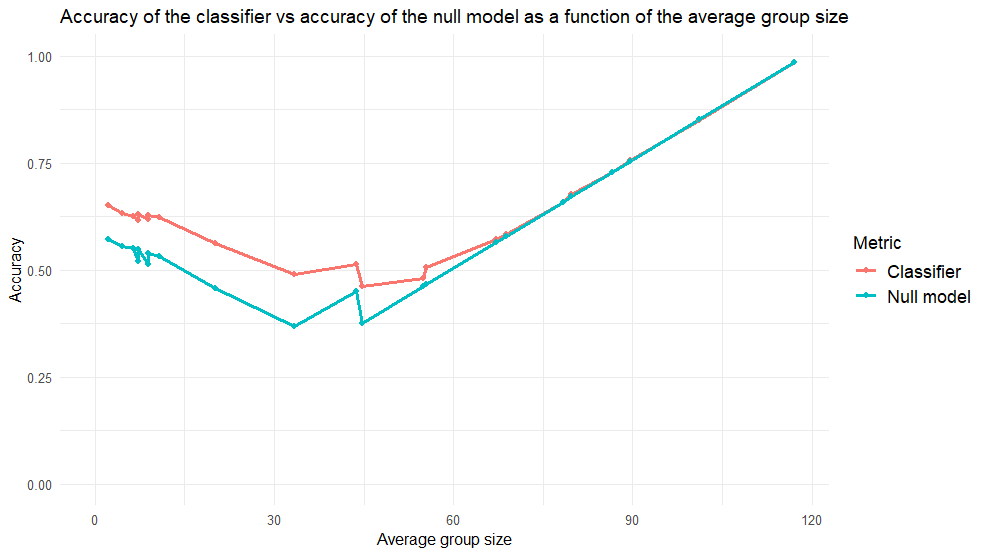
\includegraphics[width=18cm]{Pictures/LORA_classification/accuracy_dh.png}
    \caption{Evolution of the mean accuracy of the classifiers and the accuracy of the null model as a function of the average group size for DH}
    \label{fig:accuracy_dh}
\end{figure}
\begin{figure}[H]
    \centering
    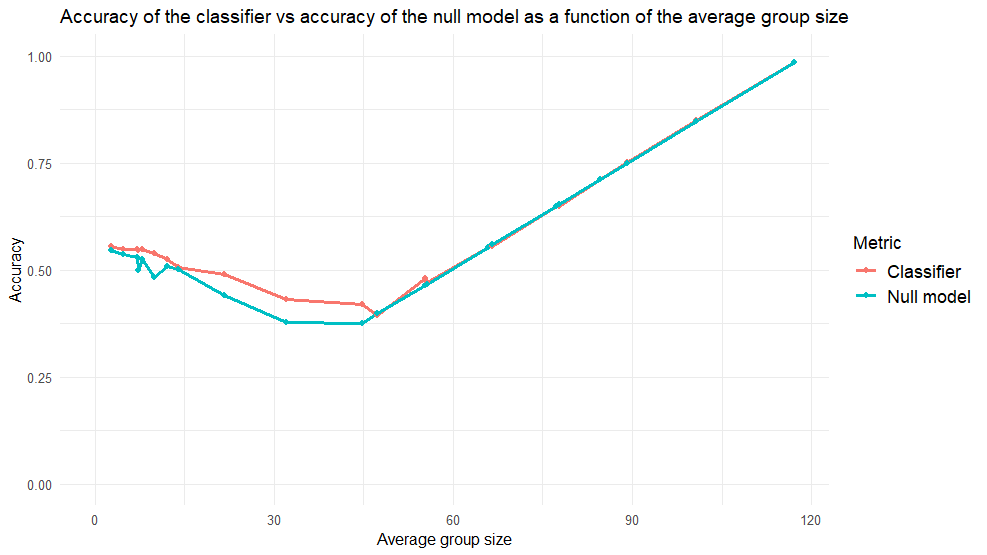
\includegraphics[width=18cm]{Pictures/LORA_classification/accuracy_pss.png}
    \caption{Evolution of the mean accuracy of the classifiers and the accuracy of the null model as a function of the average group size for PSS}
    \label{fig:accuracy_pss}
\end{figure}

In addition, we focused on classification methods that preserved a dominant average group, consistent with our conceptualization of resilience and vulnerability as deviations from the normative response. Within this constraint, we prioritized identifying resilient individuals and therefore examined the precision and recall for the resilient class.\\
\\
Figures~\ref{fig:precision_recall_dh} and~\ref{fig:precision_recall_pss} show that none of the classifiers achieved both high precision and high recall for the resilient class. In particular, no method exceeded 0.5 on both metrics simultaneously. Some classification schemes yielded high precision scores, such as the 1SD threshold for DH and the 10\% quantile method for PSS, which both exceeded 0.75, but these were associated with very low recall (below 0.1), indicating poor sensitivity to identifying resilient individuals.\\
\\
More balanced results were obtained with the 30\% quantile method (for both adversity measures) and the k-means approach applied to the PSS residuals. These yielded moderate values for both precision and recall, though still below ideal performance thresholds.
\begin{figure}[H]
    \centering
    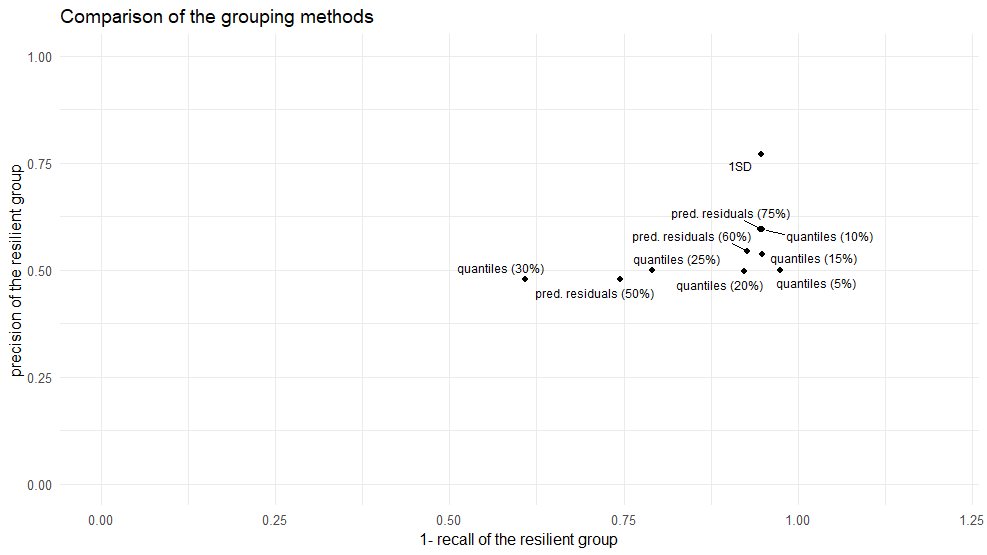
\includegraphics[width=18cm]{Pictures/LORA_classification/resilient_precision_recall_dh.png}
    \caption{Recall and precision of classifiers for the DH model}
    \label{fig:precision_recall_dh}
\end{figure}
\begin{figure}[H]
    \centering
    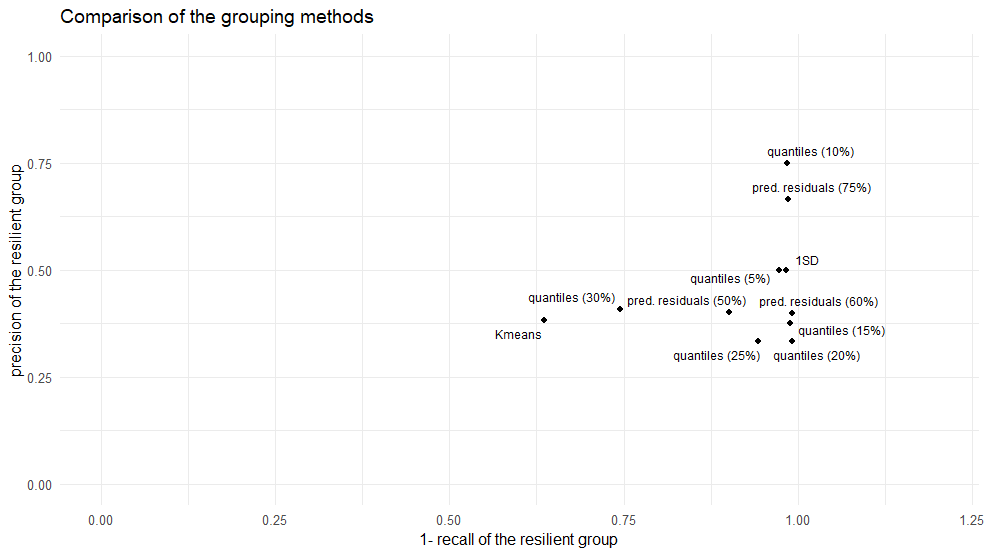
\includegraphics[width=18cm]{Pictures/LORA_classification/resilience_recall_precision_pss.png}
    \caption{Recall and precision of classifiers for the PSS model}
    \label{fig:precision_recall_pss}
\end{figure}
Overall, the results highlight the difficulty in predicting resilience and vulnerability.
\section{Longitudinal Analysis}
\subsection{Methods}
The goal of this approach is to estimate which individuals consistently deviate from the mean trajectory over time, and therefore can be categorized as resilient or vulnerable depending on the sign of the deviation. As in the cross-sectional context, we use residualization to obtain individual-level measures of resilience. Specifically, at each time point, we fit a linear regression model in which an outcome variable is regressed on an adversity variable, and we use the residuals as the resilience indicator. Again, to ensure robustness, we exclude overly influential individuals from each regression based on Cook’s distance with the same $\frac{4}{n}$ threshold (where $n$ is the number of participants). This procedure is repeated independently at each time point.\\
\\
To model the resilience across time, we then fit a linear mixed-effects model to the residuals, with both fixed effects (capturing the mean trend over all individuals) and individual-level random intercepts. These random intercepts represent persistent deviations from the average trajectory (i.e., stable individual differences in resilience).\\
\\
To identify which individuals deviate significantly from the average trajectory, we apply the method introduced by \cite{spike_and_slab}, which relies on a Bayesian \textit{spike-and-slab} prior structure. This method estimates the probability that each individual's random effect differs from zero. Using this estimated probability, after setting a threshold, individuals below the threshold are classified as average, and individuals above the threshold are classified as resilient or vulnerable, depending on the sign of the deviation.\\
\\
The \textit{spike-and-slab} method models the random effect distribution as a mixture of two components:
\begin{itemize}
  \item a \textit{spike}, corresponding to a distribution concentrated at zero, representing individuals with no stable deviation;
  \item a \textit{slab}, a more diffuse distribution around zero, representing individuals with non-zero random effects.
\end{itemize}
An indicator variable determines, for each MCMC sample, whether an individual is assigned to the spike or slab component. The proportion of MCMC samples in the \textit{slab} is then used to approximate the posterior inclusion probability (PIP), i.e. the probability that the random effect deviates from zero, and that the individual consistently deviates from the mean and therefore is non-average. Individuals with PIPs below a set threshold are classified as average, while those exceeding the threshold are classified as either resilient or vulnerable, depending on the sign of their random effect.\\
\\
Note that it is necessary to specify the prior inclusion probability in the \textit{slab}, set between 0 and 1, which controls the selectivity of the model: a value of 0.5 reflects an absence of initial hypothesis on the presence of effects, while a higher value reflects a prior belief in the existence of non-zero effects.

\subsection{Illustrative Example: LORA Project}
\subsubsection{Data and Variables}
For this illustrative example, we used again the data from the Longitudinal Resilience Assessment (LORA) project, but this time we used multiple time-points.\\
\\
For our analysis, we restricted the sample to \( N = 515 \) individuals who had completed all of the first \( T = 12 \) quarterly assessments. Again, the Perceived Stress Scale (PSS) and the Daily Hassles questionnaire (DH) were used as adversity variables, and the General Health Questionnaire (GHQ) was used as the outcome variable. The scales and coding of these variables are described in Table~\ref{table:variables_lora}.

\subsubsection{Software}
All models were implemented in \texttt{R} (version~4.4.3) using the packages \texttt{dplyr} (version~1.1.4), \texttt{rjags} (version~4.17), and \texttt{SSranef} (version~0.1.0). We fitted the models using the \texttt{ss\_ranef\_alpha()} function with its default settings, specifically:
\begin{itemize}
    \item 1,000 burn-in iterations,
    \item 1,000 sampling iterations for parameter estimation,
    \item 4 parallel MCMC chains,
    \item prior inclusion probabilities set to 0.5 for all individuals.
\end{itemize}


\subsubsection{Results}
The spike-and-slab method proved to be applicable and coherent in this longitudinal setting. Posterior inclusion probabilities (PIPs) were obtained for each individual, and group membership was assigned based on whether an individual’s PIP exceeded a chosen threshold. \\
\\
The posterior inclusion probabilities spanned a wide range. For the $GHQ\sim DH$ model, the PIPs ranged from 0.23 to 1.00, with a median of 0.52 and a mean of 0.58. For the $GHQ \sim PSS$ model, the range was 0.27 to 1.00, with a median of 0.44 and a mean of 0.55. These distributions confirm that most individuals were neither clearly average or non-average, and that the classification is sensitive to the choice of PIP threshold.\\
\\
Figures~\ref{fig:PIP_pss} and~\ref{fig:PIP_dh}, along with Tables~\ref{table:PIP_pss} and~\ref{table:PIP_dh}, show the evolution of group sizes as the PIP threshold increases for the $GHQ\sim PSS$ and $GHQ\sim DH$ models, respectively. In both models, increasing the PIP threshold leads to fewer individuals being classified as non-average, as expected.\\
\\
A small asymmetry between the resilient and vulnerable groups was observed in both models. For the $GHQ\sim PSS$  model, the vulnerable group was consistently slightly larger than the resilient group across all PIP thresholds. In contrast, for the $GHQ\sim DH$ model, the resilient group was slightly larger than the vulnerable group up to a threshold of 0.9, after which the trend reversed.\\
\\
These results confirm that the method is sensitive to the user-defined PIP threshold, while producing stable and interpretable classifications that are, however, slightly asymmetrical between the two non-average groups.\\
\\
Figures~\ref{fig:visu-threshold-dh} and~\ref{fig:visu-threshold-pss} display the mean residuals of each group across the 12 time points, for different selected PIP thresholds. As the threshold increases, the mean residuals of the resilient and vulnerable groups move further away from zero. This pattern reflects the fact that higher thresholds assign non-average status only to individuals with more extreme and consistent deviations from the normative trajectory, thereby increasing group separation but also reducing group size, as seen previously.


\begin{table}[H]
\centering
\rowcolors{2}{gray!20}{white}
{\small
\begin{tabular}{>{\centering\arraybackslash}p{1cm}
>{\centering\arraybackslash}p{4cm}
>{\centering\arraybackslash}p{4cm}
>{\centering\arraybackslash}p{4cm}}
\hline
PIP & Percentage atypical & Percentage resilient & Percentage vulnerable \\
\hline
0.50 & 45.44 & 21.55 & 23.88 \\ 
0.55 & 40.39 & 19.03 & 21.36 \\ 
0.60 & 36.70 & 16.50 & 20.19 \\ 
0.65 & 33.79 & 14.76 & 19.03 \\ 
0.70 & 31.07 & 13.79 & 17.28 \\ 
0.75 & 27.77 & 12.04 & 15.73 \\ 
0.80 & 24.47 & 11.07 & 13.40 \\ 
0.85 & 19.61 & 8.16 & 11.46 \\ 
0.90 & 16.70 & 6.99 & 9.71 \\ 
0.95 & 14.56 & 6.02 & 8.54 \\ 
1.00 & 6.60 & 1.94 & 4.66 \\ 
\hline
\end{tabular}
}
\caption{Proportions of individuals in each category depending on the chosen PIP threshold for GHQ $\sim$ PSS}
\label{table:PIP_pss}
\end{table}

\begin{figure}[H]
    \centering
    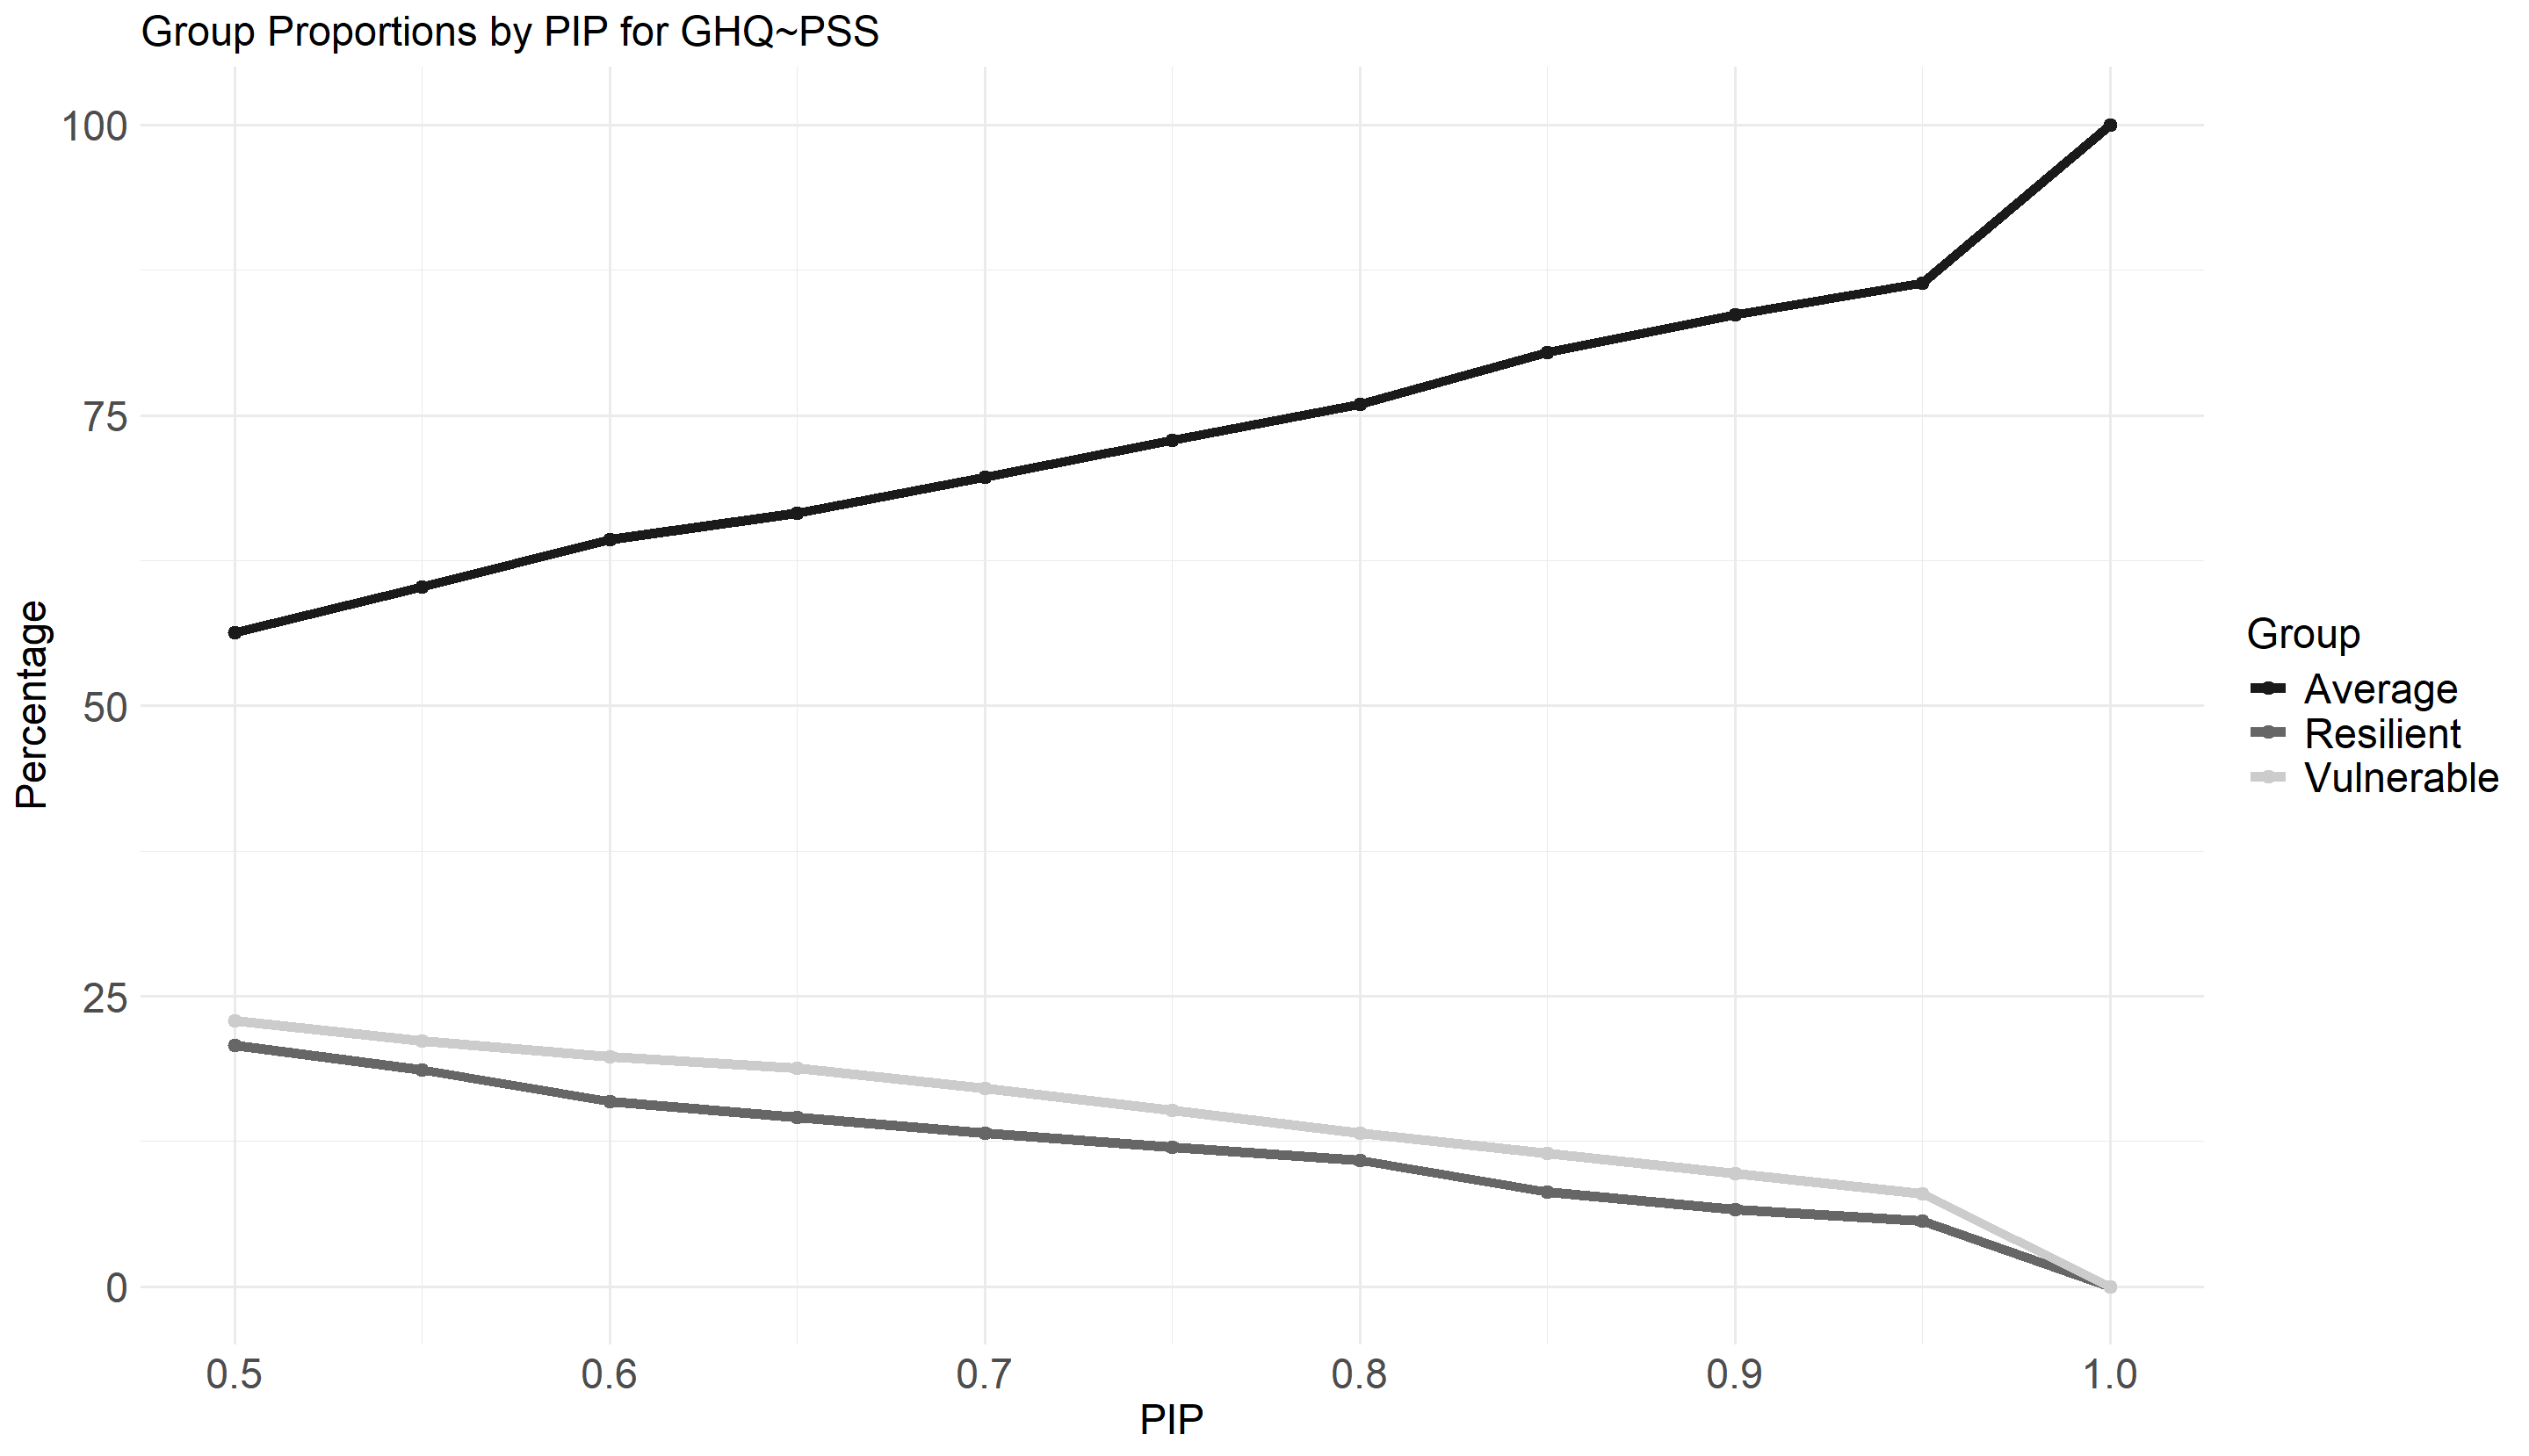
\includegraphics[width=18cm]{Pictures/longitudinal/PIP_pss.png}
    \caption{Proportions of individuals in each category depending on the chosen PIP threshold for GHQ $\sim$ PSS}
    \label{fig:PIP_pss}
\end{figure}

\begin{table}[H]
\centering
\rowcolors{2}{gray!20}{white}
{\small
\begin{tabular}{>{\centering\arraybackslash}p{1cm}
>{\centering\arraybackslash}p{4cm}
>{\centering\arraybackslash}p{4cm}
>{\centering\arraybackslash}p{4cm}}
\hline
PIP & Percentage atypical & Percentage resilient & Percentage vulnerable  \\
\hline
0.50 & 52.43 & 28.54 & 23.88 \\ 
0.55 & 47.77 & 26.60 & 21.17 \\ 
0.60 & 43.50 & 24.27 & 19.22 \\ 
0.65 & 40.58 & 23.11 & 17.48 \\ 
0.70 & 37.86 & 21.17 & 16.70 \\ 
0.75 & 35.73 & 19.81 & 15.92 \\ 
0.80 & 32.62 & 17.86 & 14.76 \\ 
0.85 & 28.74 & 14.95 & 13.79 \\ 
0.90 & 26.21 & 12.82 & 13.40 \\ 
0.95 & 20.58 & 9.51 & 11.07 \\ 
1.00 & 11.46 & 4.27 & 7.18 \\ 
\hline
\end{tabular}
}
\caption{Proportions of individuals in each category depending on the chosen PIP threshold for GHQ $\sim$ DH}
\label{table:PIP_dh}
\end{table}

\begin{figure}[H]
    \centering
    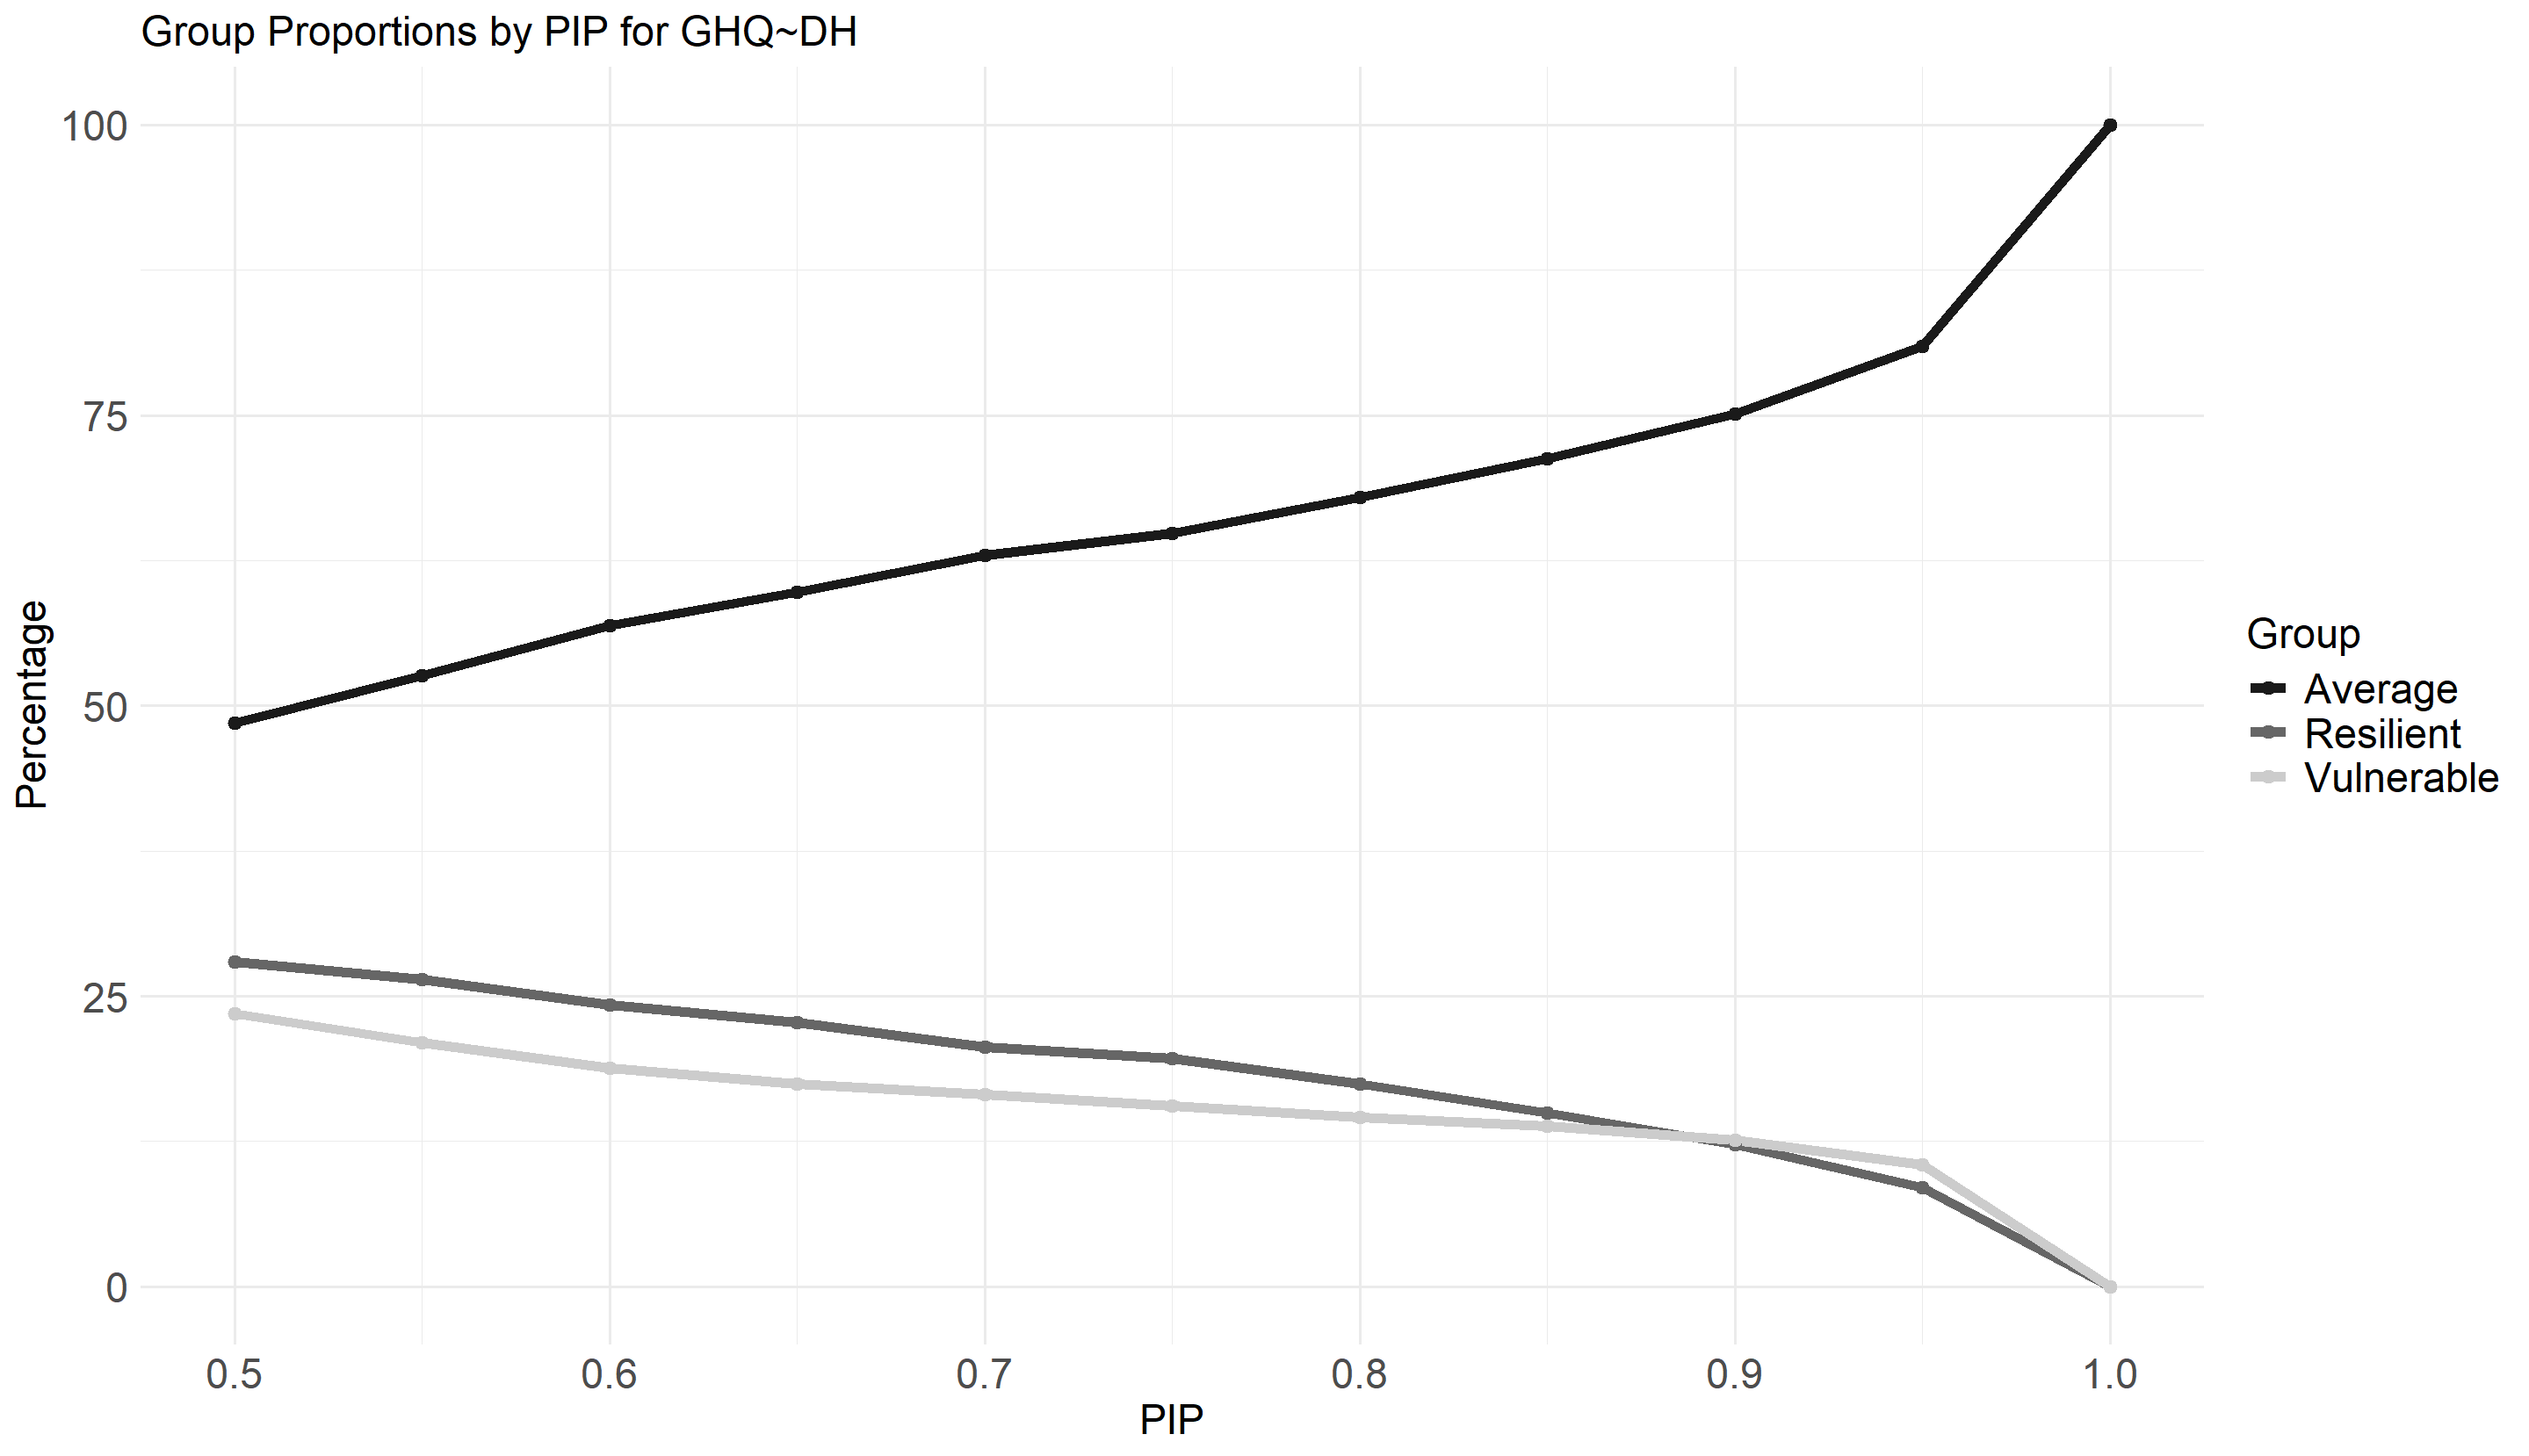
\includegraphics[width=18cm]{Pictures/longitudinal/PIP_dh.png}
    \caption{Proportions of individuals in each categories depending on the chosen PIP threshold for GHQ $\sim$ DH}
    \label{fig:PIP_dh}
\end{figure}

\begin{figure}[H]
    \centering
    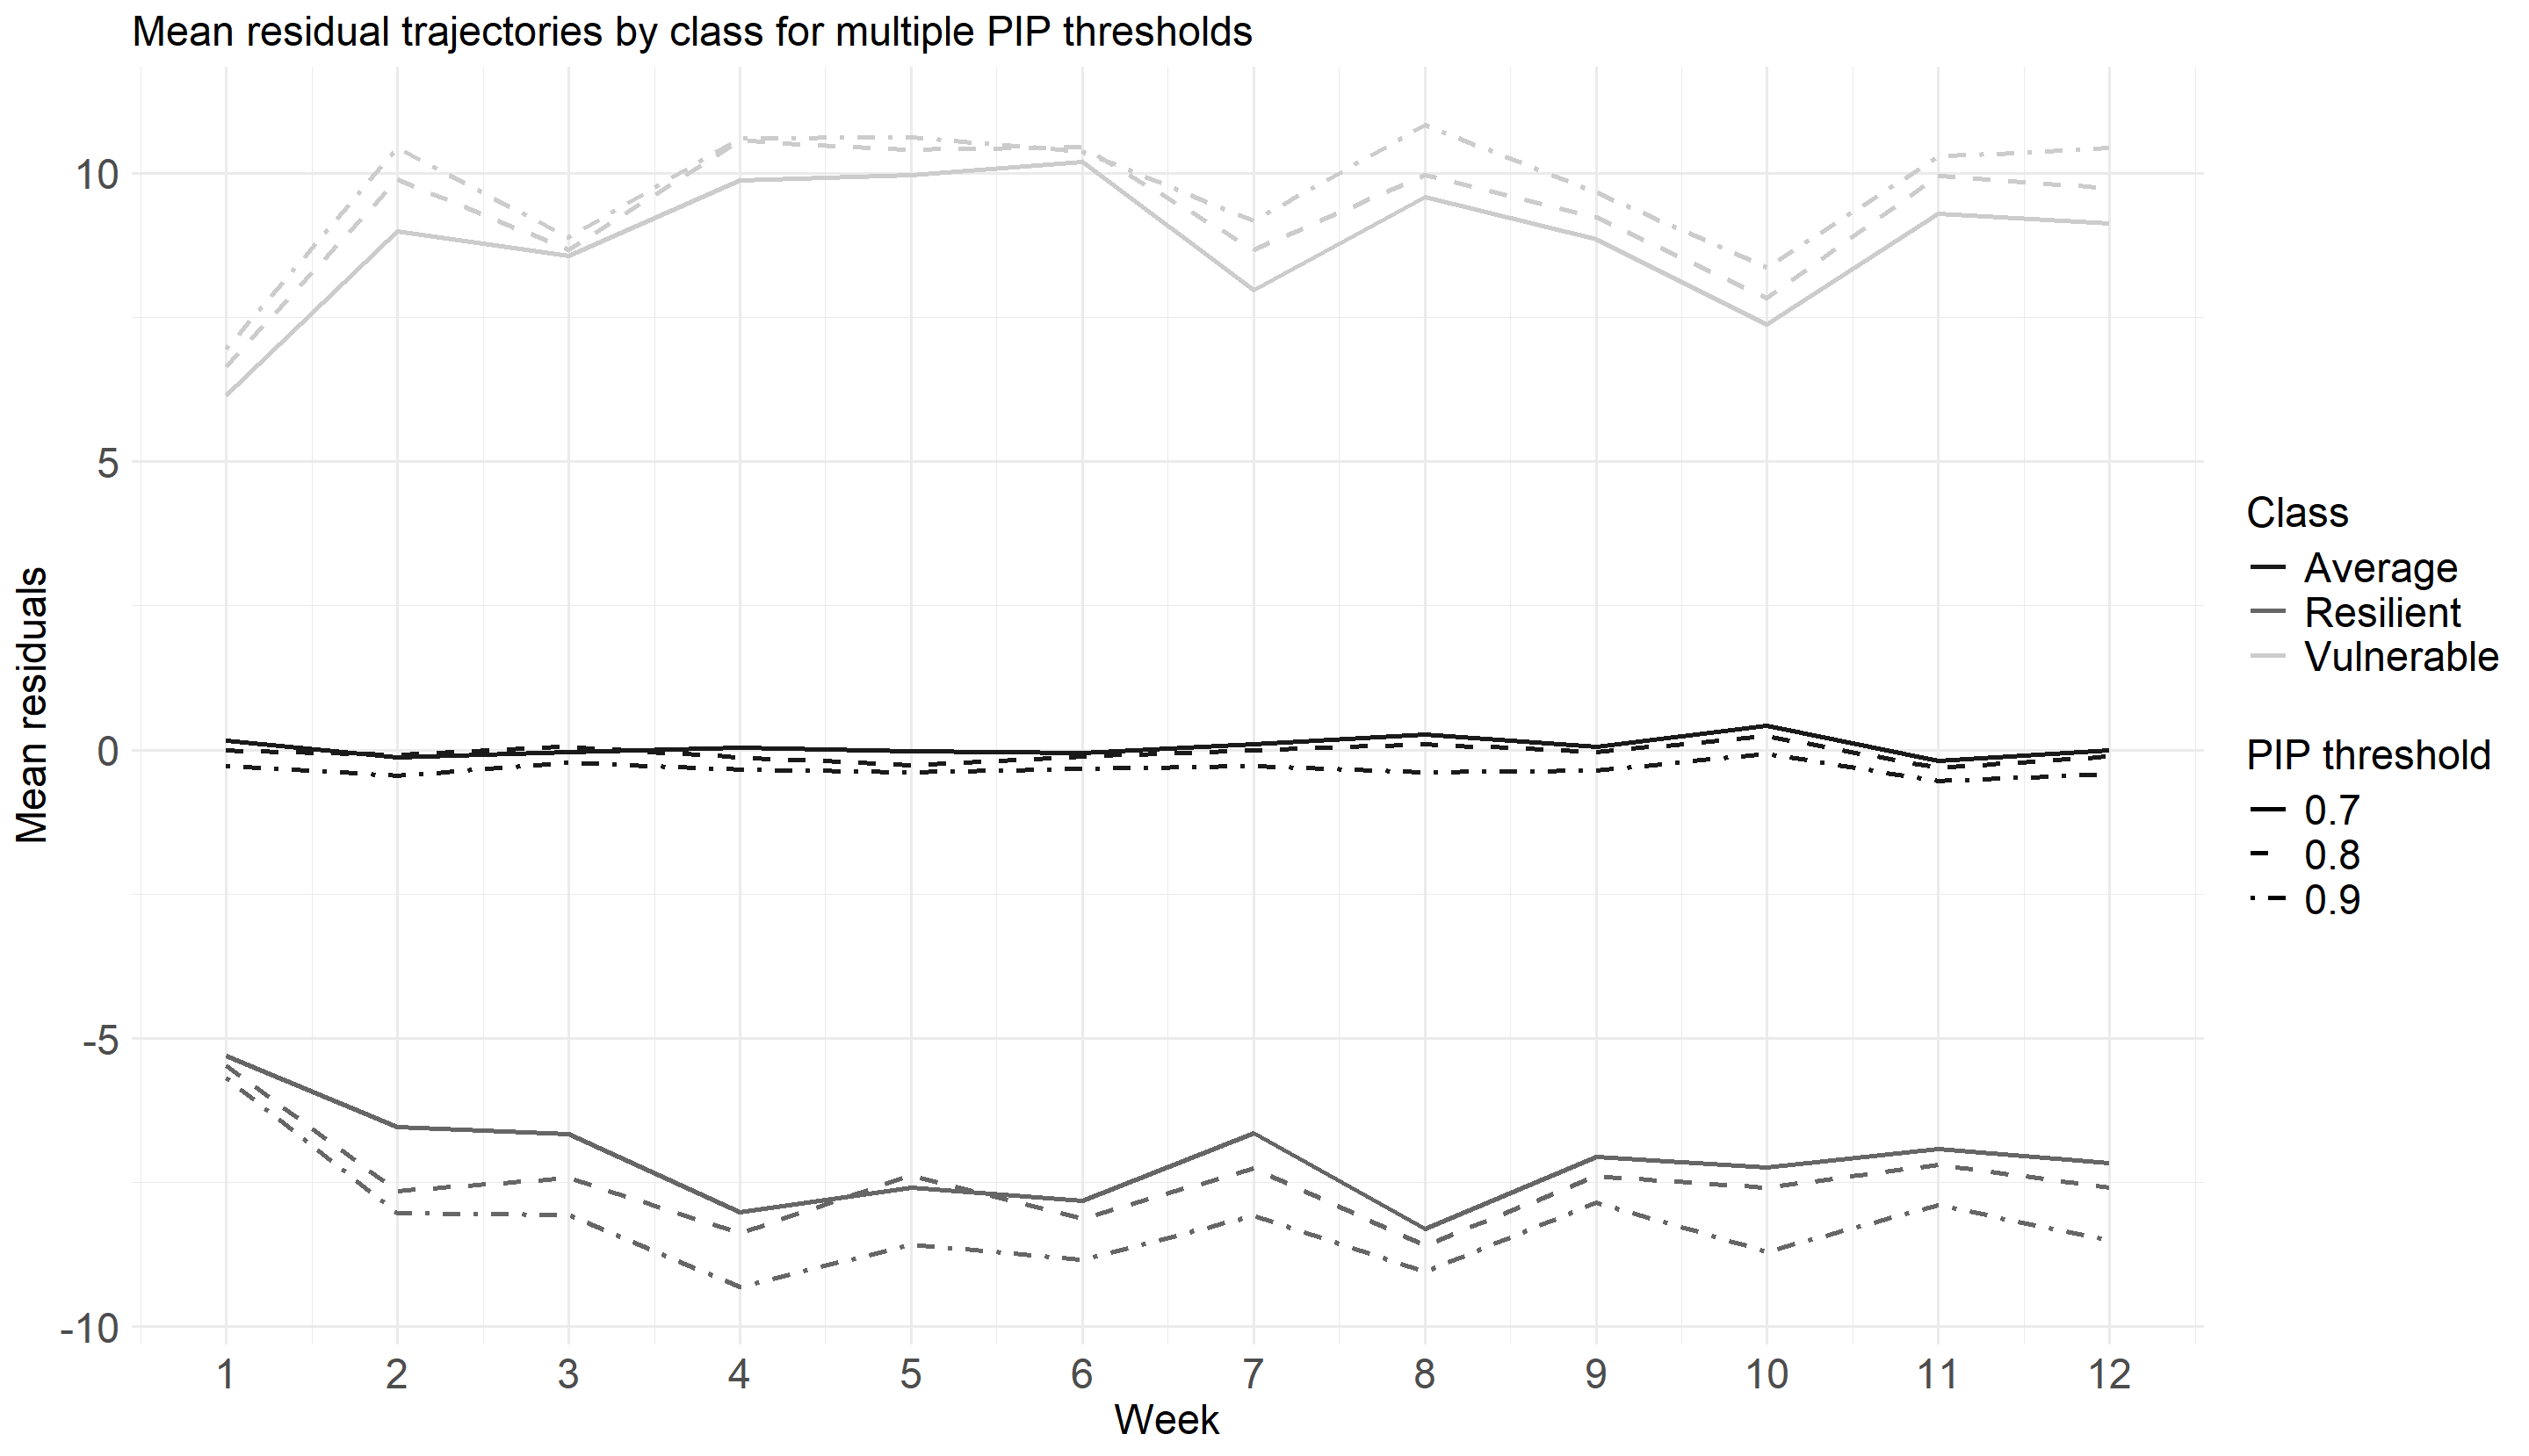
\includegraphics[width=18cm]{Pictures/longitudinal/visualization_thresholds_dh.png}
    \caption{Evolution of the mean residuals for each group using different thresholds to build the groups for DH}
    \label{fig:visu-threshold-dh}
\end{figure}

\begin{figure}[H]
    \centering
    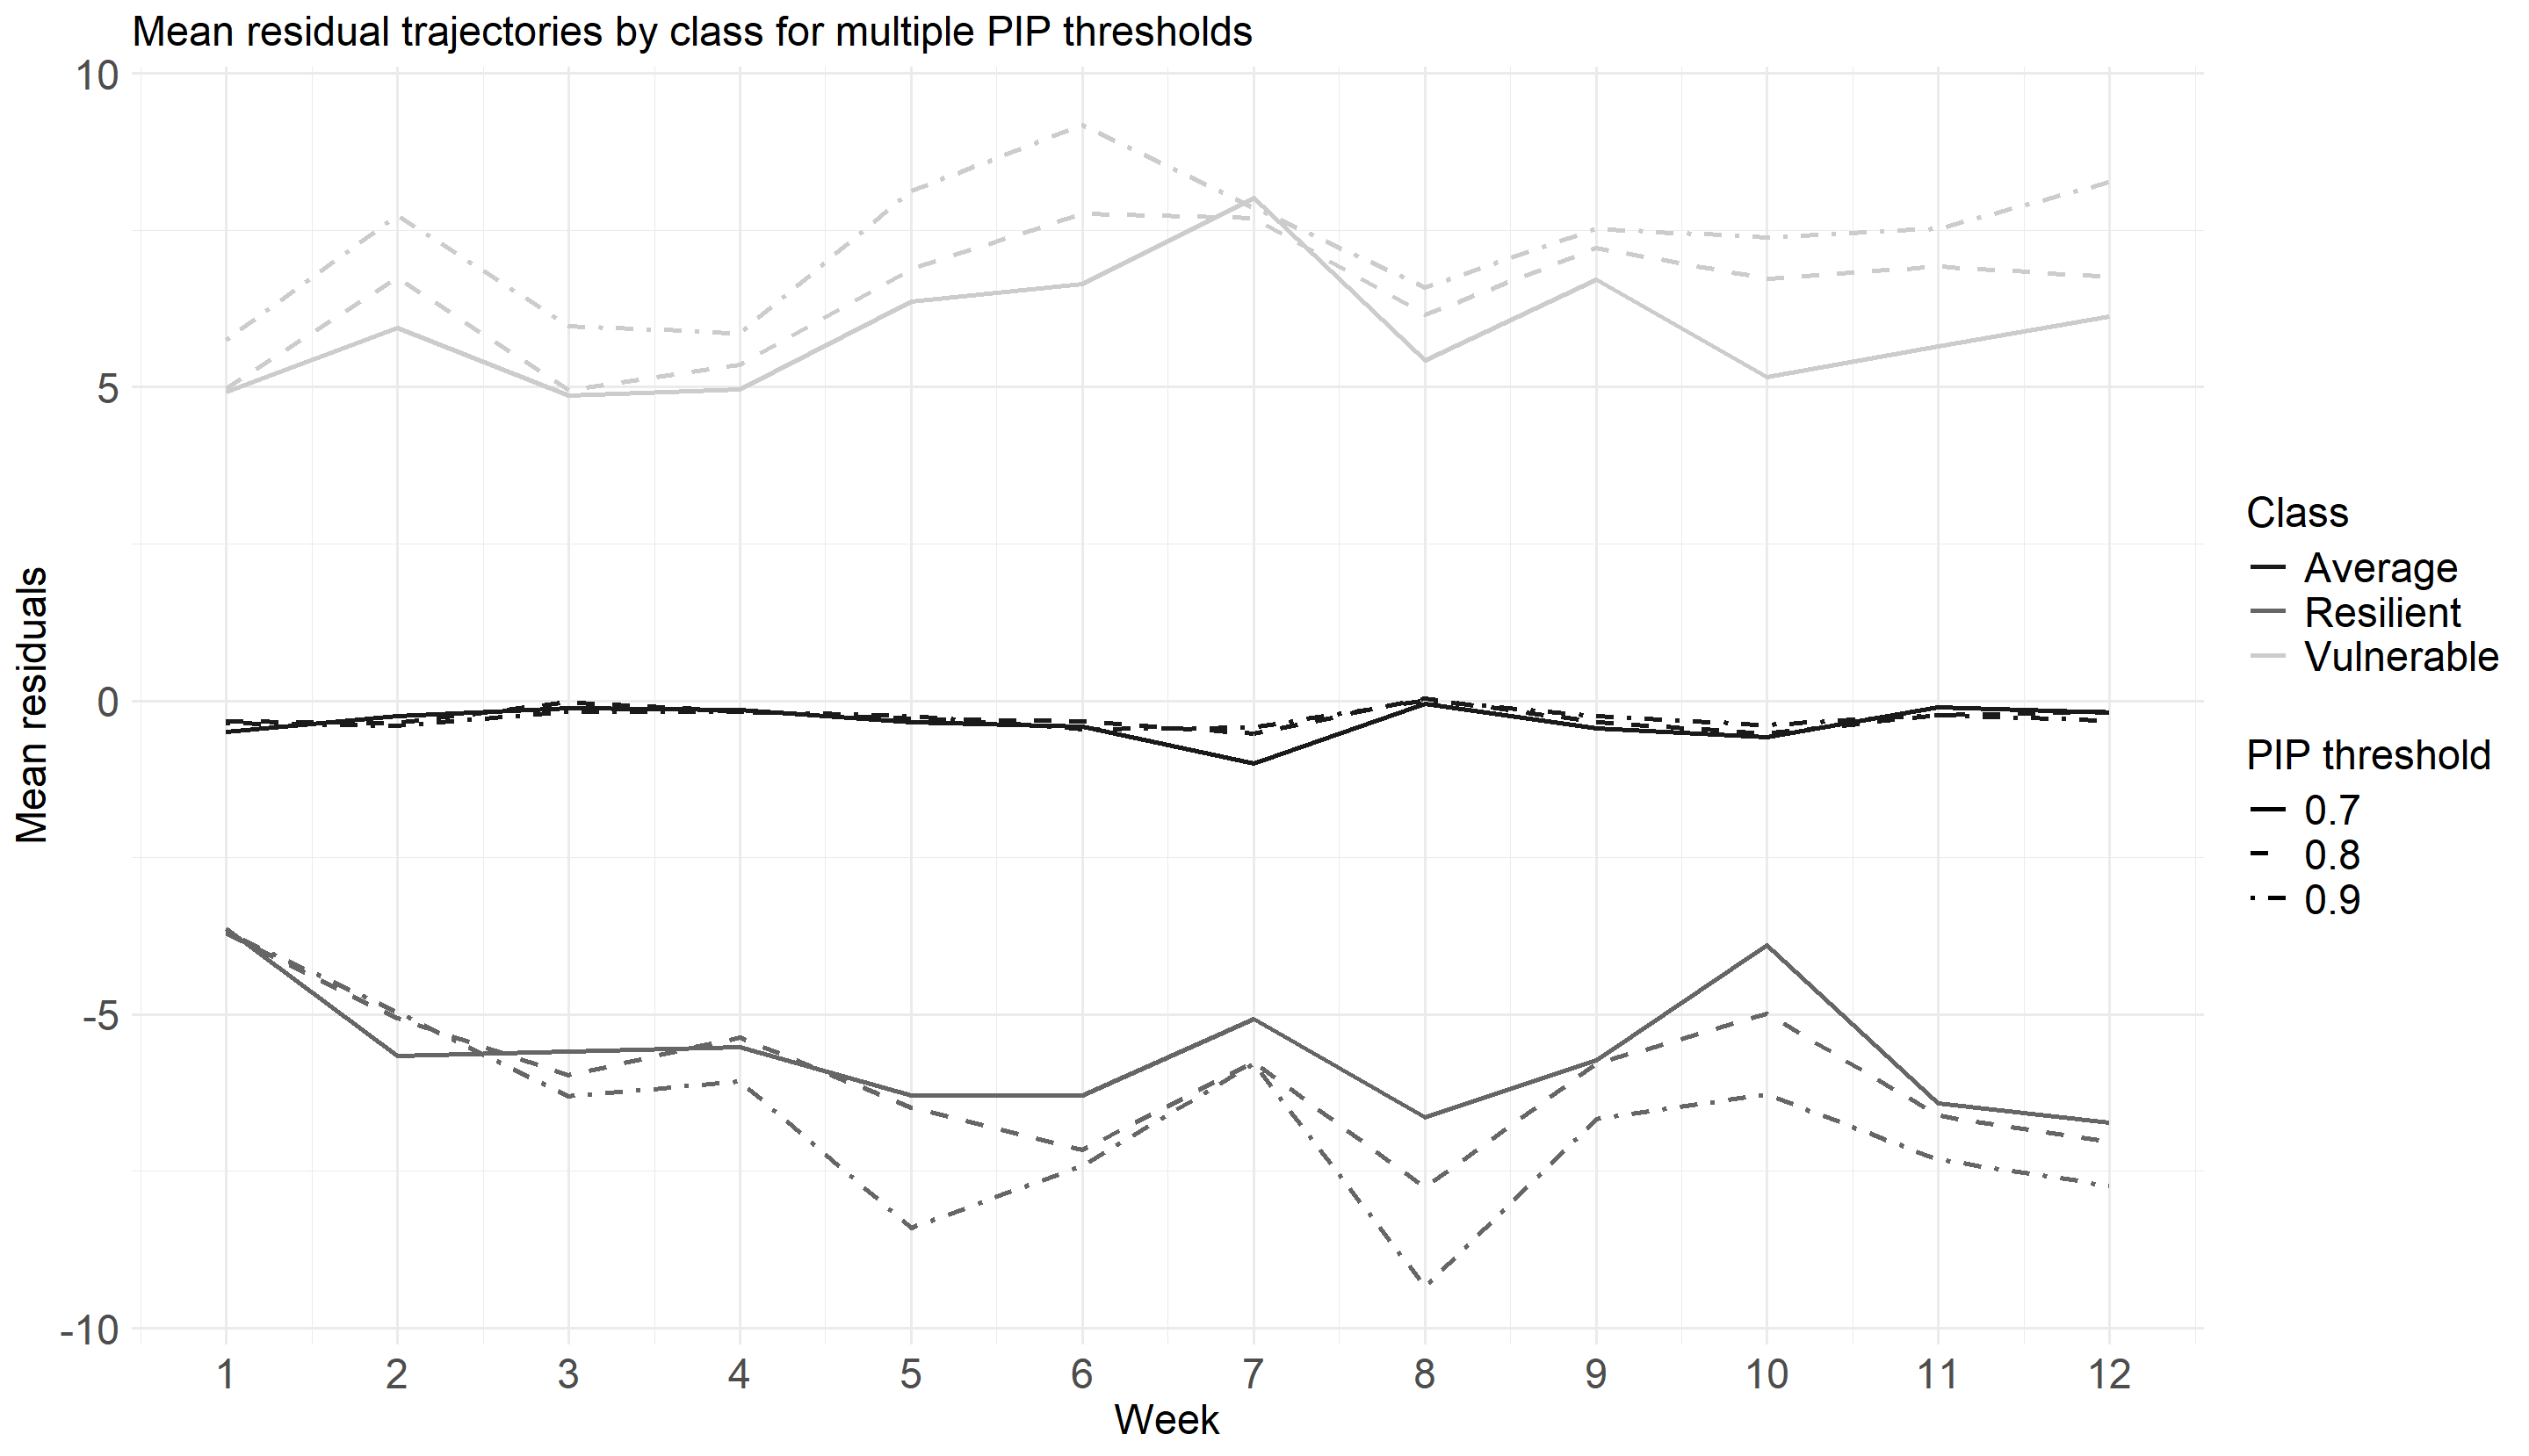
\includegraphics[width=18cm]{Pictures/longitudinal/visualization_thresholds_pss.png}
    \caption{Evolution of the mean residuals for each group using different thresholds to build the groups for PSS}
    \label{fig:visu-threshold-pss}
\end{figure}


\newpage
\addcontentsline{toc}{section}{References}
\printbibliography

\end{document}
